%!TEX root = ../doc.tex
\chapter{Testing and Results}
\label{sec:Results}
The following chapter describes the calibration, testing and the results of the system components. 
\section{ToF Camera}
The time-of-flight camera is the crucial part of this thesis, allowing a three-dimensional scene reconstruction. This section describes the measurements and the results of the motion estimation of the ToF Camera at every involved step.
\subsection{Setup}
As described in section \ref{sec:camHead}, the ToF camera sends its data by ethernet, using a lightweight TCP protocol. The software controlling the setup of the ToF camera runs on the Raspberry Pi and is the proprietary part of the ToF software stack. The software allows a basic configuration in two main modes: automatic and manual control. The software supports HDR functionality in both automatic and manual control, which significantly enhances the dynamic range on the infrared black-and-white image. The implementation of the HDR function is not documented by the supplier of the Nimbus 3D ToF camera.\\ 
The ToF camera uses an infrared flash, which is not brightness-controlled; setting the camera to a fixed exposure time would lead to overexposure on close objects. The automatic mode lets the user select a maximum amplitude of the image, to which the exposure time is set. As the CudaSift library, which extracts the SIFT features from the ToF camera, only supports the 8-bit resolution, the maximum amplitude got selected at 255. Higher values lead to a longer exposure time and let the frame rate drop. Not needing any amplitude scaling while keeping a high frame rate is favorable. 
\begin{figure}[H]
    \centering
    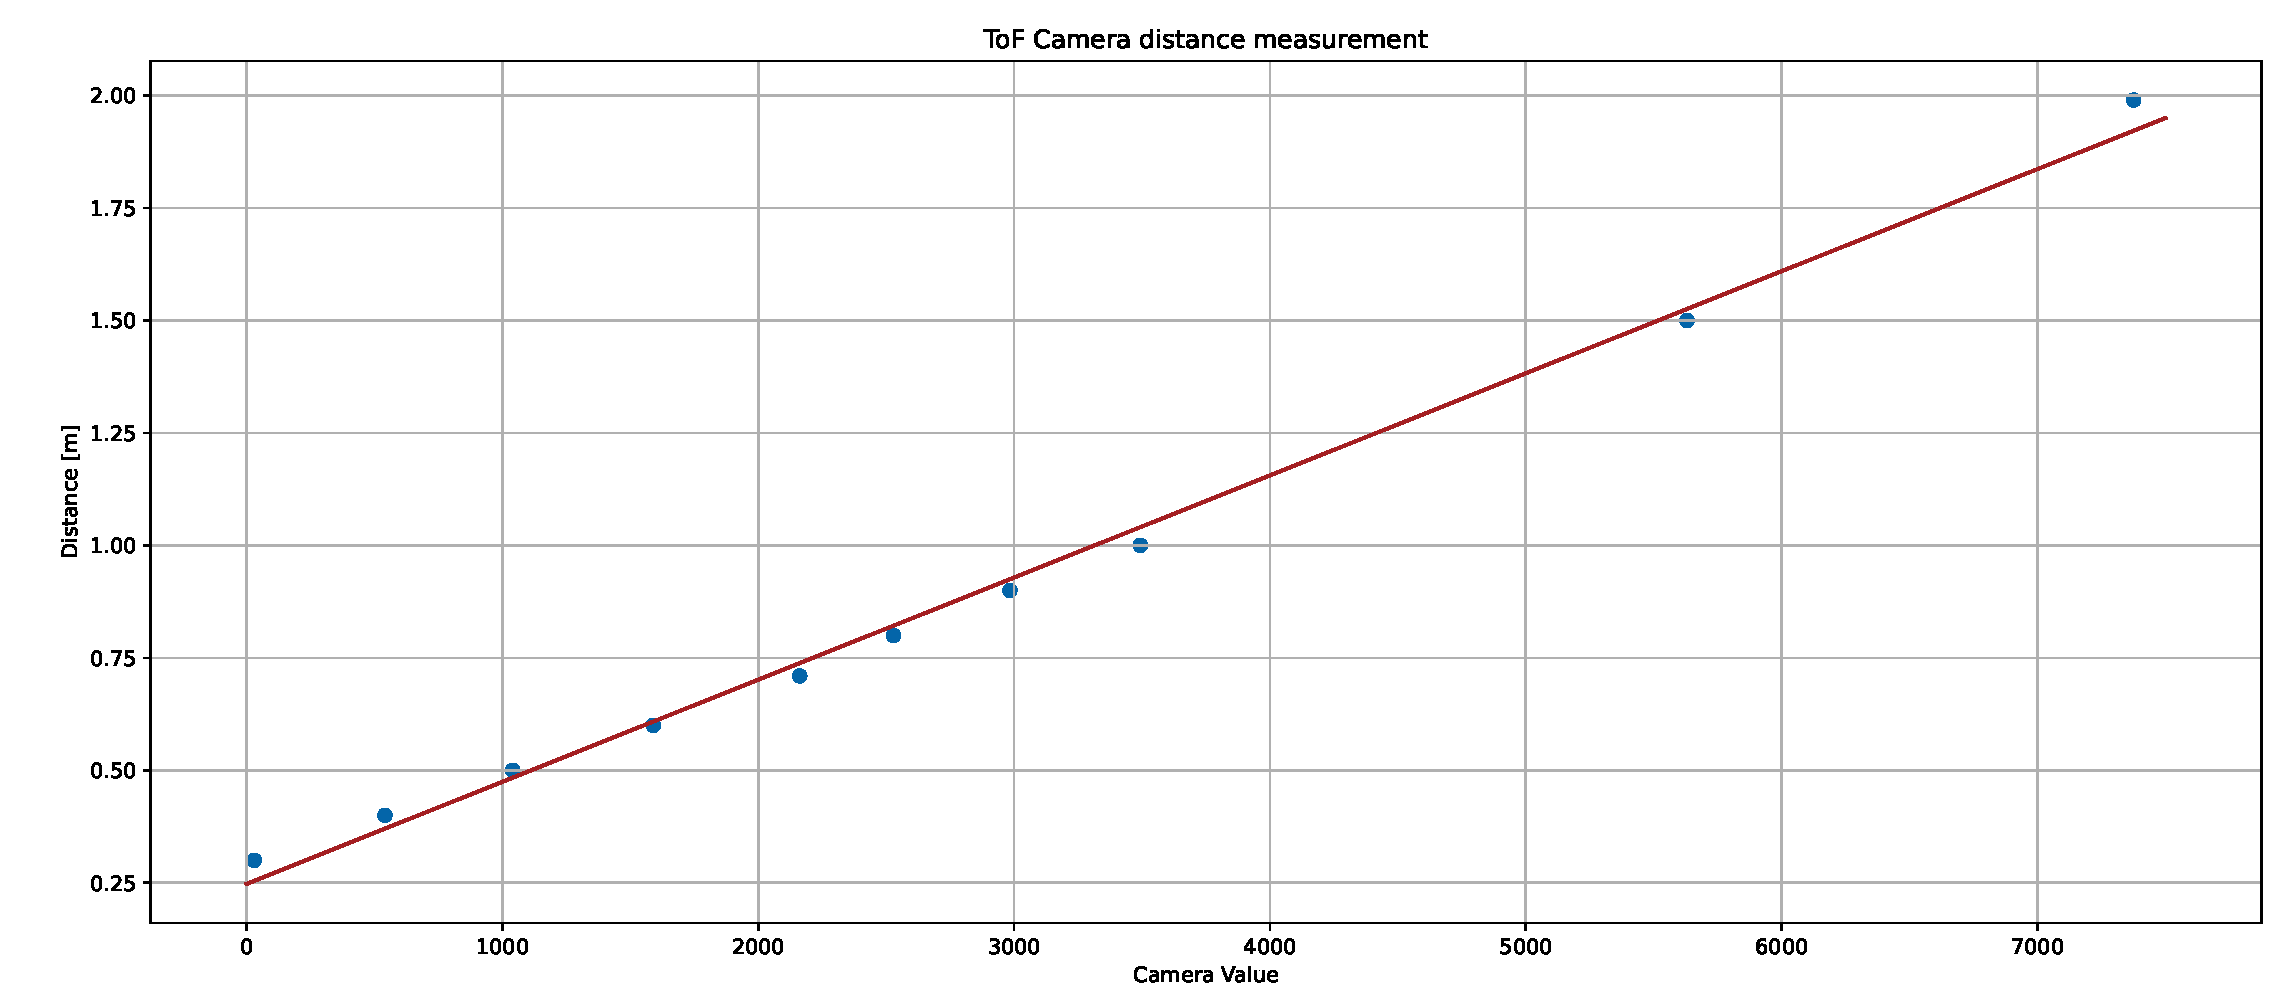
\includegraphics[width=1.0\textwidth]{images/camera_distance_measurement.eps}
    \caption{Sensor values measured against a meterstick. In red, the linear fit generated in Microsoft Excel.}
    \label{im:distance_measurement}
\end{figure}
The coordinate system is not corrected for $x$, $y$ and $z$ yet, as the ToF camera itself does not know its rotation in the field of gravity. Therefore, the axis for the ToF camera calculations are kept in the $a$, $b$ and $c$ system. Details are explained in section \ref{sec:ABC_XYZ_coords}.
\subsection{Distance measurement}
\label{sec:results_distance_meas}
Every pixel of a ToF camera sensor combined with the wide-area infrared flash acts like a laser rangefinder. A single pixel of the sensor targeting a brown cardboard surface positioned at various distances allows measuring this distance with a meterstick and a comparison with the sensor pixel value. A linear fit in Microsoft Excel leads to the following function, which is also visualized in image \ref{im:distance_measurement}:
\begin{equation*}
    d [m] = 0.000227 * val +0.247532
\end{equation*}
The camera noise does affect not only the black-and-white image but also the distance measurement. At the chosen camera settings, the camera noise lets the distance measurement have a standard deviation of around 7mm in the $a$-axis.\\
The formulae for the 3D scene reconstruction propagate the standard deviation to about 4mm in the $b$-axis and 3mm in the $c$-axis.
\subsection{3D Scene Reconstruction}
After calibrating the lens and correcting the radial nature of the distance measurement as described in section \ref{sec:ToFCalibration}, the generated point cloud should directly reconstruct the three-dimensional scene recorded by the ToF camera. Section \ref{sec:ToFPosition_SIFT} describes the process of this reconstruction.
Straight lines in the real world should appear straight in the point cloud, which can be checked by analyzing an image. The two images in figure \ref{fig:linearity3d} demonstrate the point cloud generation, by mapping SIFT features into the 3D space. 
\begin{figure}[H]
    \centering
    \begin{minipage}[b]{0.45\textwidth}
      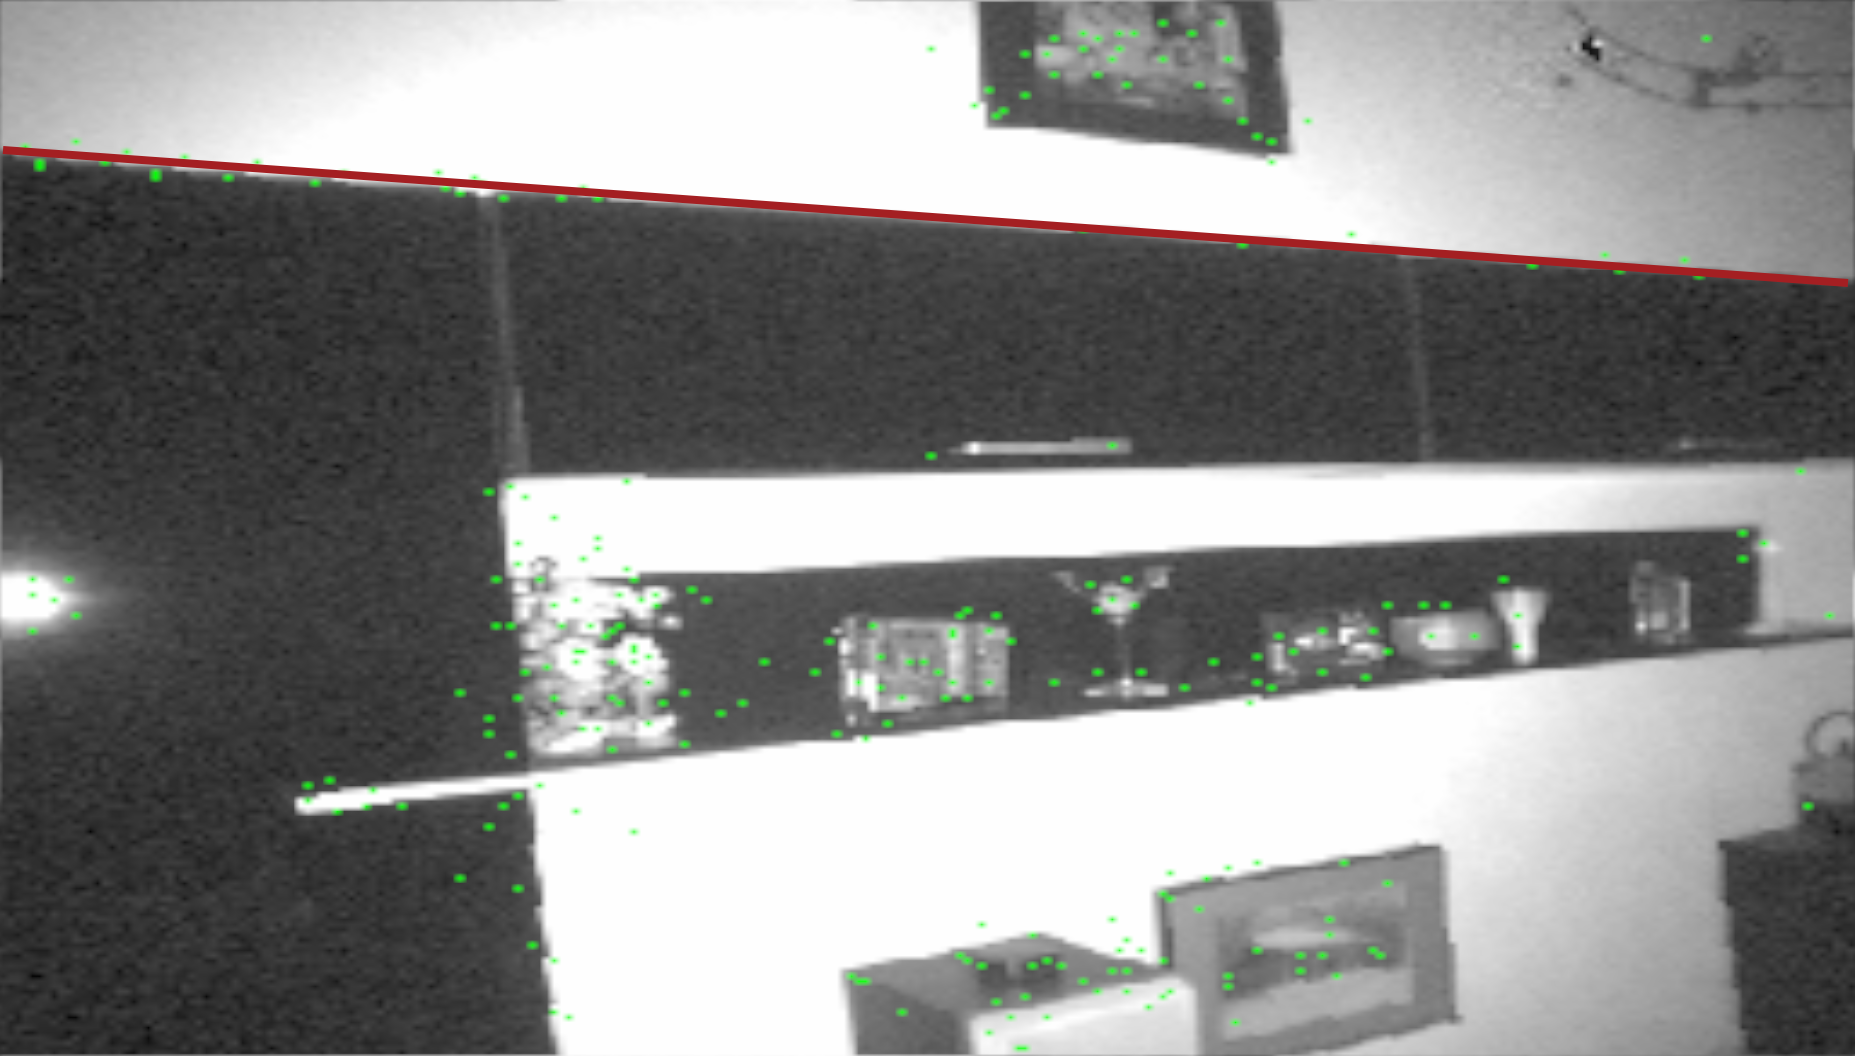
\includegraphics[scale=0.105]{images/cloud_3d_linearity_image.png}
      \caption{Image}
      \label{fig:linearity3d_image} 
    \end{minipage} % Hier darf keine Leerzeile zwischen den beiden Minipages liegen!
    \begin{minipage}[b]{0.45\textwidth}
      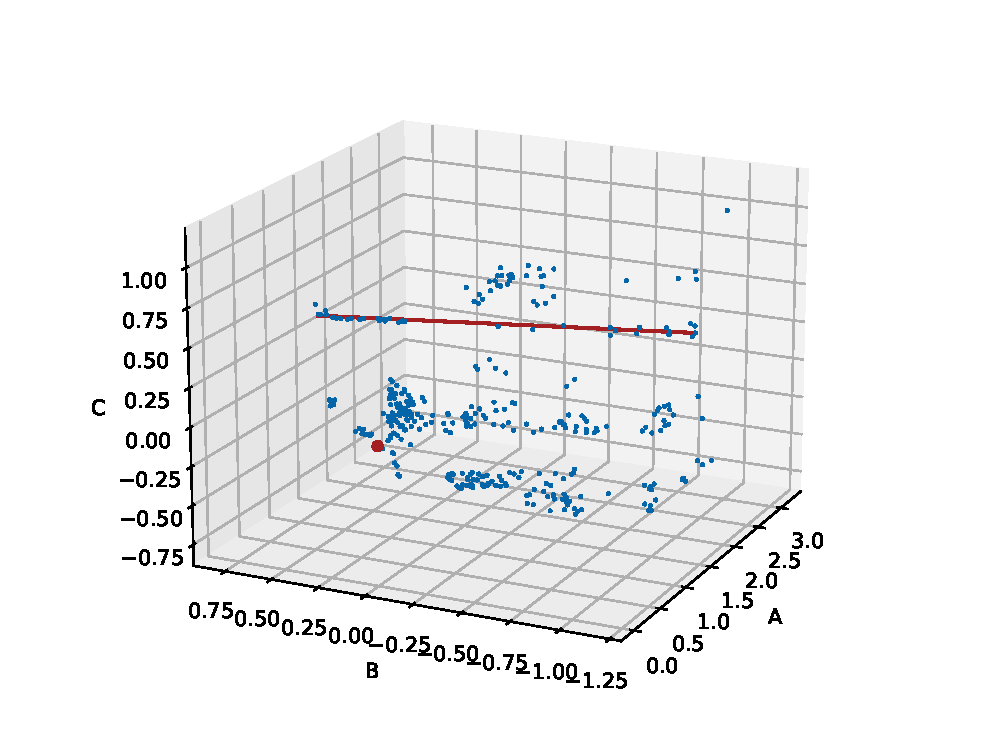
\includegraphics[scale=0.45, trim={0cm 0cm 2cm 3.5cm},clip]{images/linearity_3d.eps} 
      \caption{Cloud}
      \label{fig:linearity3d_cloud} 
    \end{minipage}
    \caption{The scene reconstruction from the left image to the full point cloud. The red line is equivalent in both figures. Each green dot in the image on the left is a SIFT feature. The red dot in the point cloud is the position of the camera.}
    \label{fig:linearity3d}
  \end{figure}
\subsection{RANSAC feature matching}
\label{sec:RANSAC_Results}
The RANSAC algorithm improves the quality of matched features over the flawed brute-force matcher. Section \ref{sec:ToFPosition_RANSAC} explains the implementation of the three-dimensional RANSAC and mentions a threshold. The noisy data the ToF camera delivers gives single SIFT features a positional uncertainty. As discussed in section \ref{sec:results_distance_meas}, the standard deviation in the $a$-axis is roughly 7mm, which also affects the mapping to the$b$- and $c$-axis from the 3d reconstruction. Therefore, the RANSAC matcher is required to have flexibility against positional noise.\\
Prior analysis of the dataset tells a possible rotation and translation. This rigid motion moves each data point in the old cloud to an estimated position, where a data point of the new cloud is expected.  The lowest sum of square differences (SSD) of all the possible matches to the estimated position determines a match. It is accepted if this matched point lies inside the chosen SSD threshold. 
The SSD creates a sphere around the estimated position. The equation of a sphere of radius $r$ follows the equation $r^{2}=x^{2}+y^{2}+z^{2}$. Setting the radius $r$ equal to the standard deviation of 7 mm on the $a$-axis results in a threshold of around 0.00005. Statistically, around 68\% of the matches should reside inside this sphere of 14 mm diameter. The error on the other axis is smaller as discussed in section \ref{sec:results_distance_meas}, this does not explain the poor matching performance at this threshold, as seen in image \ref{im:noise_against_thresh}. Because of the image noise on the black-and-white image, the extracted SIFT features jitter. Even a jitter in the range of 1 pixel easily leads - depending on its distance - to an error of more than a centimeter. On the other hand, to detect a lateral speed of 0.1 m/s at a frame rate of approximately 10 frames per second, a shift of 1 cm needs to be detected.
\begin{figure}[H]
    \centering
    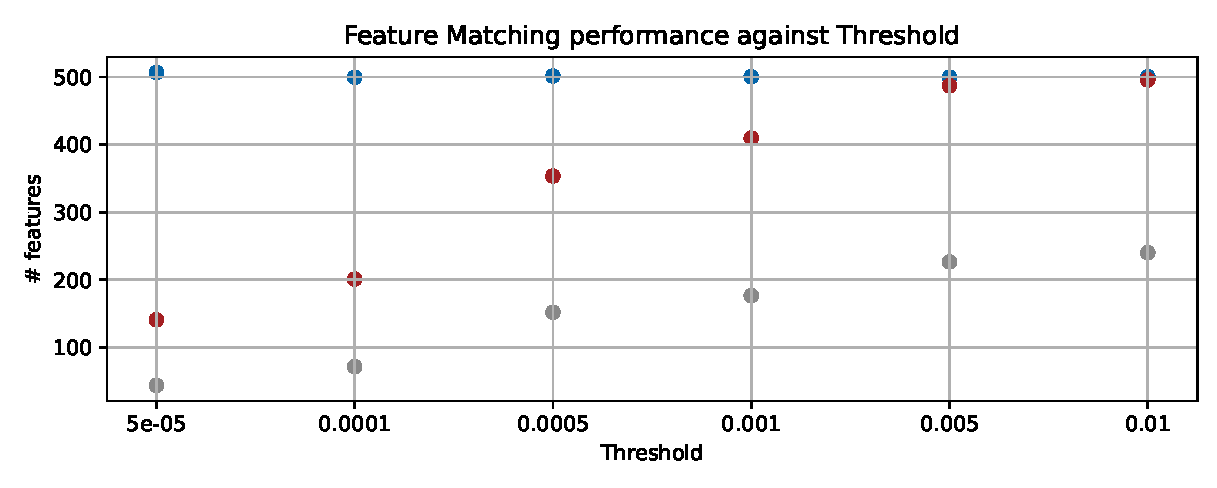
\includegraphics[width=1.0\textwidth]{images/noise_against_threshold.eps}
    \caption{Plotting the feature matching performance against different thresholds shows the quality of the RANSAC feature matcher. In blue, the raw number of unmatched features in each test, in gray the brute force matches and in red the RANSAC matches.}
    \label{im:noise_against_thresh}
\end{figure}
Higher tresholds in image \ref{im:noise_against_thresh} show the expected performance of the brute-force matcher in grey, which lies below 50\% according to the developers of the CudaSift library.\cite{cudaSiftRepo} The RANSAC feature detector vastly improves the matching performance, seemingly up to over 97\% at the threshold of 0.005. At the threshold of 0.005, the sphere around the expected position measures over 14 cm in diameter. The RANSAC matcher might find the same match for different feature points; its matches are not exclusive, combined with the large threshold, it is likely that most features find a match.\\
The balance between the uncertainty and the requirements for detecting slow speeds lead to a chosen threshold of 0.0005. This threshold leads to a sphere of about 4.4 cm in diameter, which filters harsh outliers.\\ 
Figure \ref{im:3d_features_rotation} on the next page demonstrates the matching with the chosen threshold at the example of a rotation of the camera head. Two consecutive frames generate a point cloud each; one is marked blue, the other in red. The estimated rotation and translation move each blue data point to a hypothetical position. The closest red data point around this hypothetical position is accepted if it lies within a sphere of 4.4cm diameter. 
After another calculation, these matched data points lead to the optimal rigid motion, discussed in the following sections.

\begin{figure}[H]
  \centering
  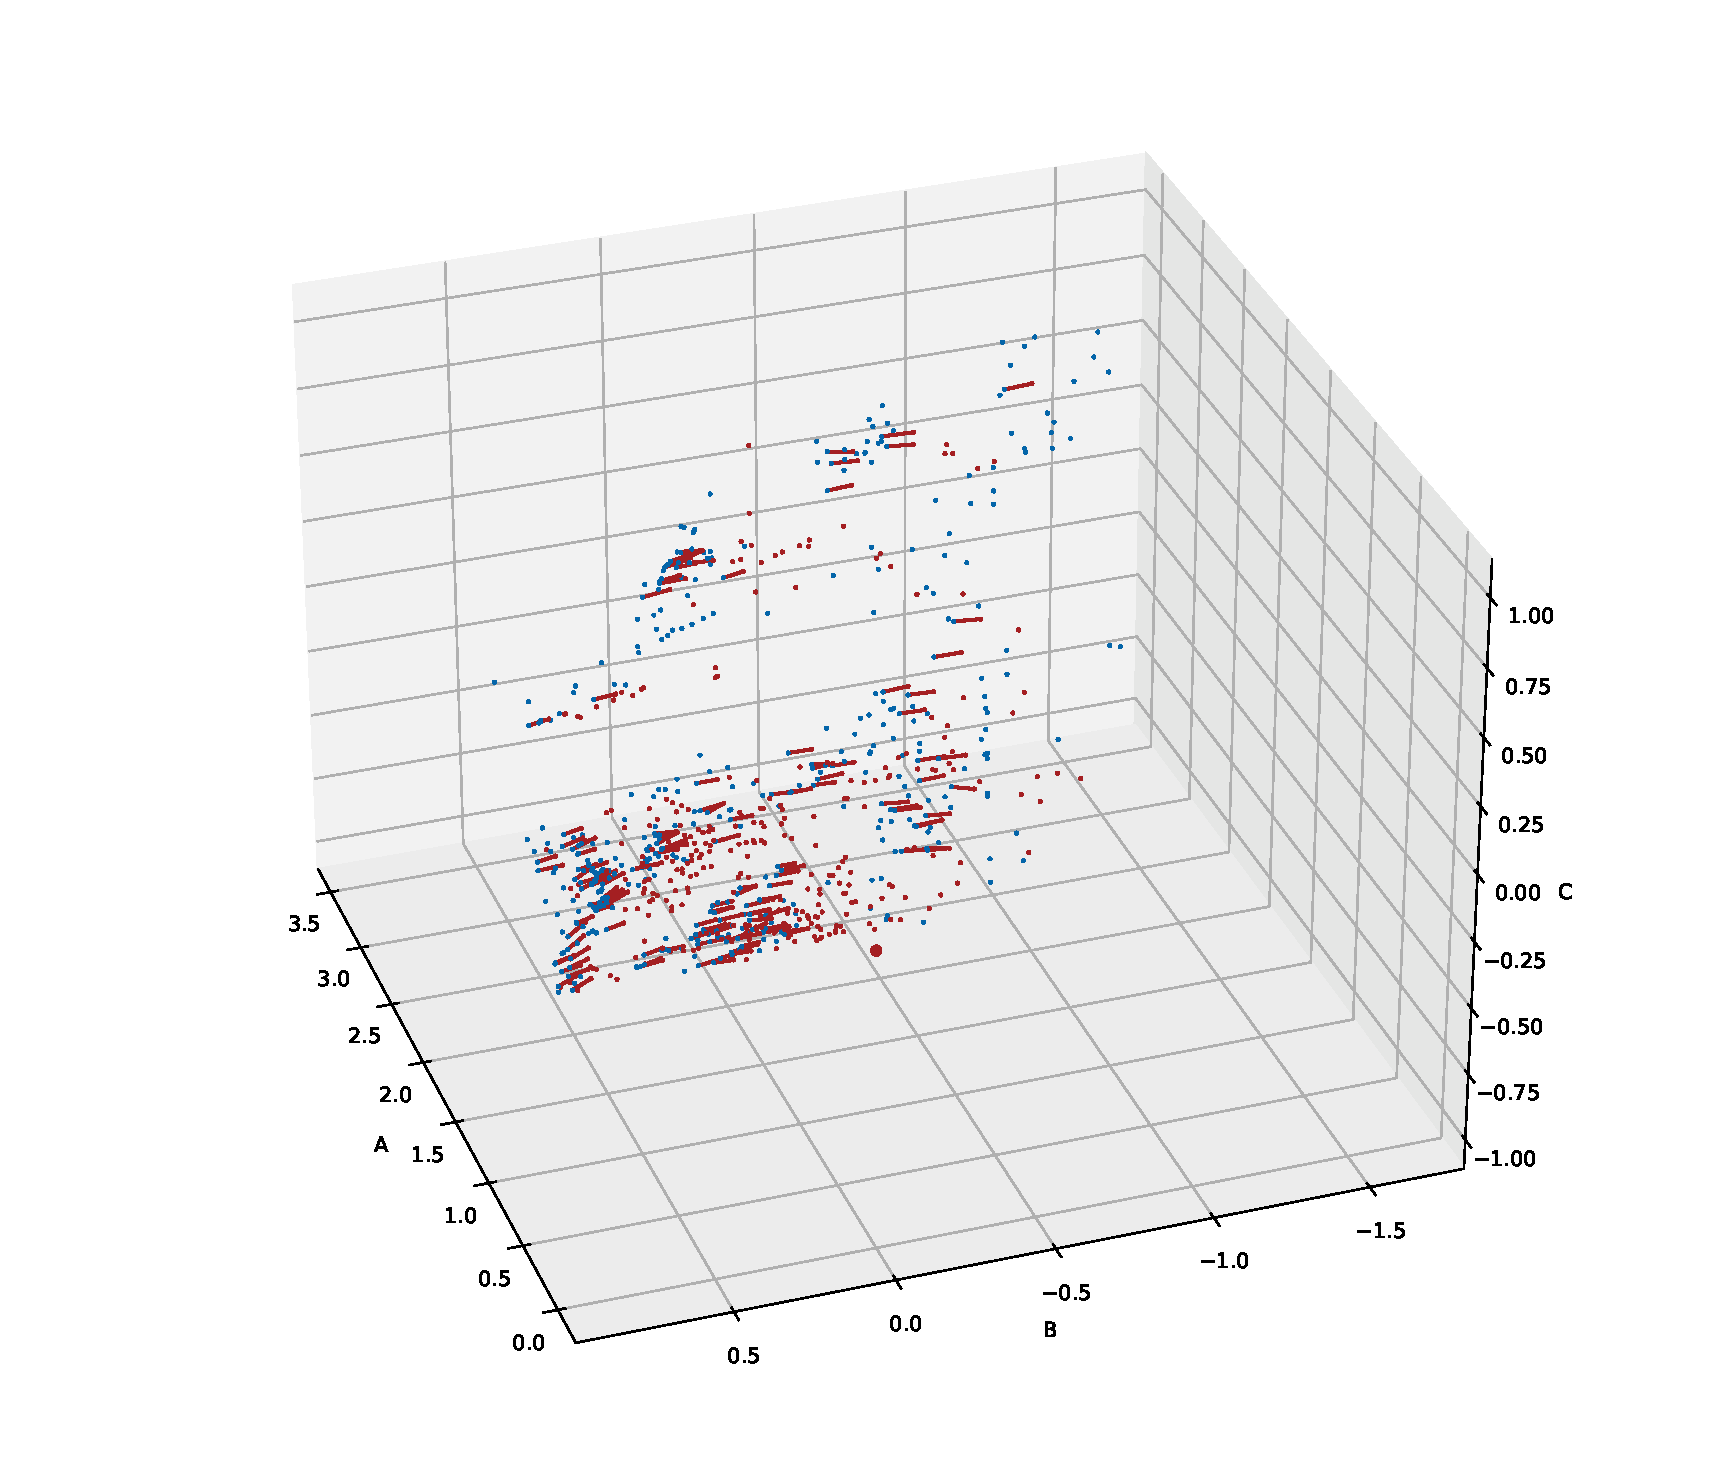
\includegraphics[width=1.0\textwidth,trim={7cm 7cm 8cm 5cm},clip]{images/3d_features_rotation.eps}
  \caption{Two raw point clouds with the found matches connecting them. The camera is rotated in between the frames, which leads to the displacement of the point cloud. The connecting lines are roughly 10cm long, depending on the position. The large red dot in the foreground is the position of the camera. The scene is the same as in image \ref{fig:linearity3d}, but zoomed for better visibility.}
  \label{im:3d_features_rotation}
\end{figure}
\subsection{Rotation from ToF camera}
\label{sec:results_tof_rotation}
The optimal rotation between the point clouds is ready for comparison against the gyroscope of the IMU. Both the gyroscope and the ToF rotation generate rotation speeds and are both converted into rotation quaternions. Transforming the rotation speed to a quaternion allows direct comparison of the different imaginary parts. In addition, the quaternions can be fed directly to the Kalman Filter. The real part of a rotation quaternion is always entirely dependent on the imaginary factors; therefore, analyzing the imaginary parts is sufficient, as explained in section \ref{sec:RotationQuaternion}.
For demonstration, the camera head gets rotated in each direction and directly compared to the gyroscope data. The author does not own a device that allows reference rotations; the camera got mounted on a standard camera tripod and rotated by hand. Figure \ref{im:tof_rotation_measurement} shows the results. First the camera head got rotated sideways around the $c$-axis, then up and down along the $b$-axis and lastly turned along the $a$-axis. The plotted values resemble imaginary parts of a quaternion and are therefore without units.
\begin{figure}[H]
  \centering
  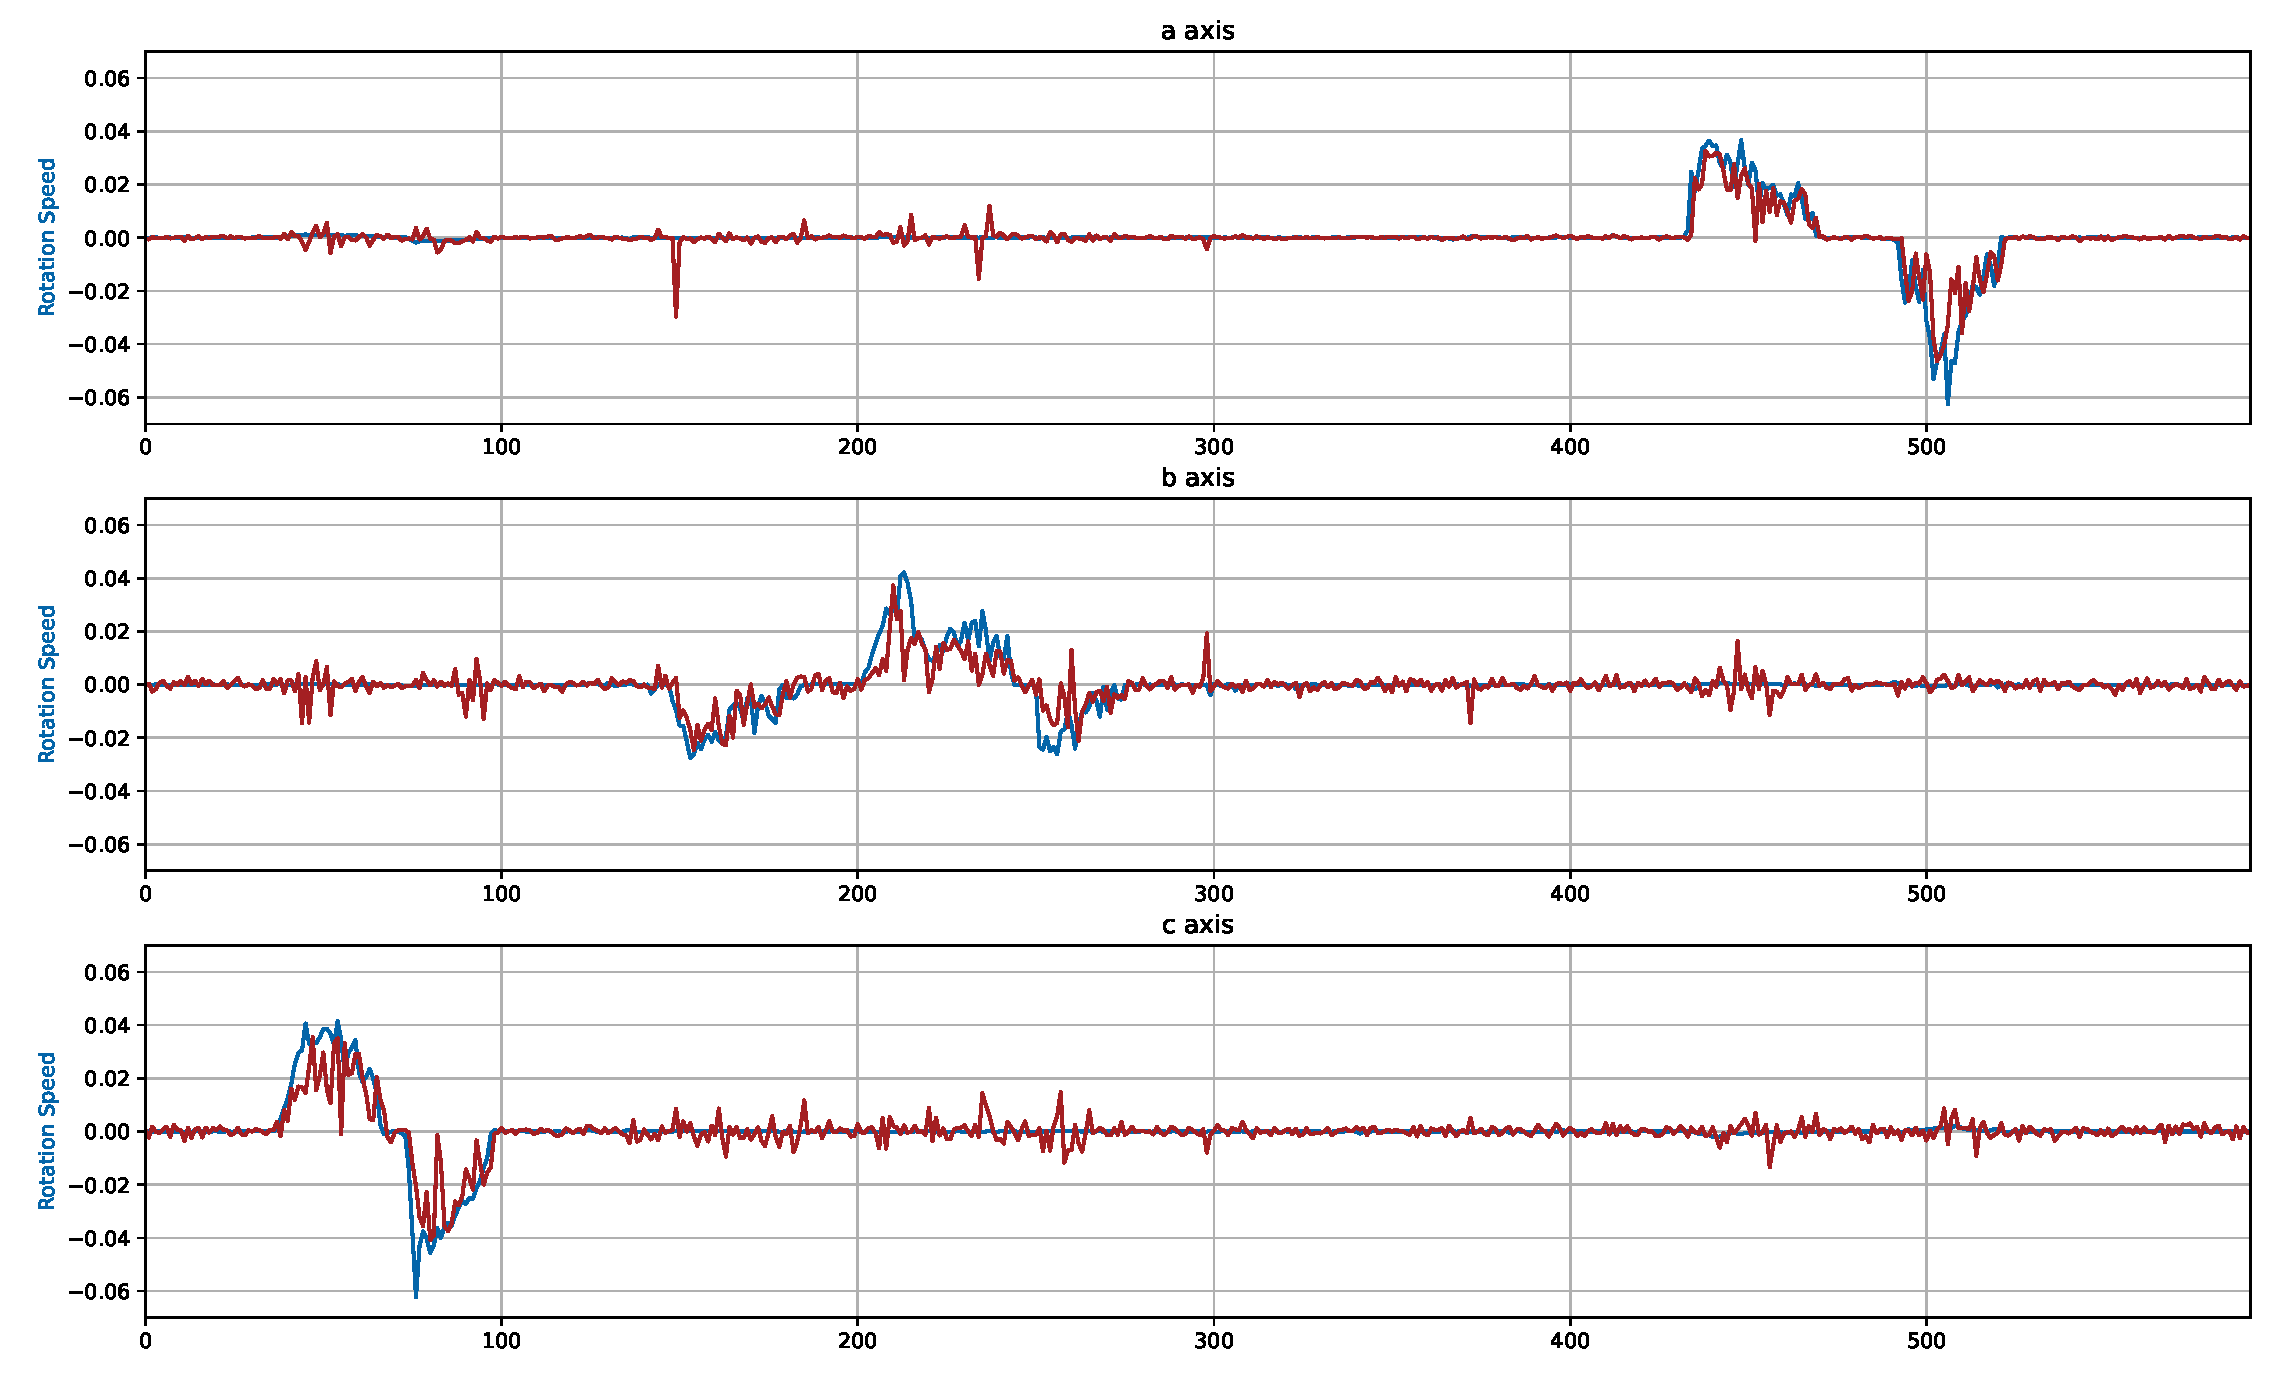
\includegraphics[width=1.0\textwidth]{images/tof_rotation_measurement.eps}
  \caption{The individual axis of the ToF rotation quaternion plotted against the gyroscope quaternion. The camera head got rotated in each direction after another.}
  \label{im:tof_rotation_measurement}
\end{figure}
The measurement shows significant noise, especially on the rotation alongside the b- and c-axis, and does not entirely follow the gyroscope curve in blue. Nevertheless, the concept works as this measurement demonstrates. 
\subsection{Translation from ToF camera}
Like for the rotation measurement, the translation is measured against the IMU. In the case of translation, the IMU only contains an accelerometer, which stands in contrast to the velocity estimated by the ToF camera. As for the rotation, the author has no device that allows standardized motion; the camera head is moved by hand.\\
A toy railway system helps guide the camera alongside the x- and y-axis. Vertical motion - along the z-axis - technically works the same as motion alongside the y-axis; it is not measured, as there is no vertical rail system at hand. The translation cannot be measured in one take as the Railway needs to be moved for the different axis.\\
Alongside the x-axis, the camera moves closer to the objects in the viewfinder, alongside the y-axis, the camera moves perpendicular. Note that these measurements are already in xyz-notation, as the orientation is corrected. As the camera does not rotate during these measurements, the values are equivalent to the abc-notation. The camera is slid from its origin to the front, respectively to the side, twice, while going back to the origin twice. The first motion is kept fast, the second motion is kept slow. The length of the track is about 0.5 m in both directions.\\
As visible in the figures \ref{im:tof_translation_measurement_x} and \ref{im:tof_translation_measurement_y} on the next page, the velocity data from the ToF camera shows significant noise, but the motion is detected correctly. The coloring of the curves is kept the same as in figure \ref{im:KalmanFilter1D}.
\begin{figure}[H]
  \centering
  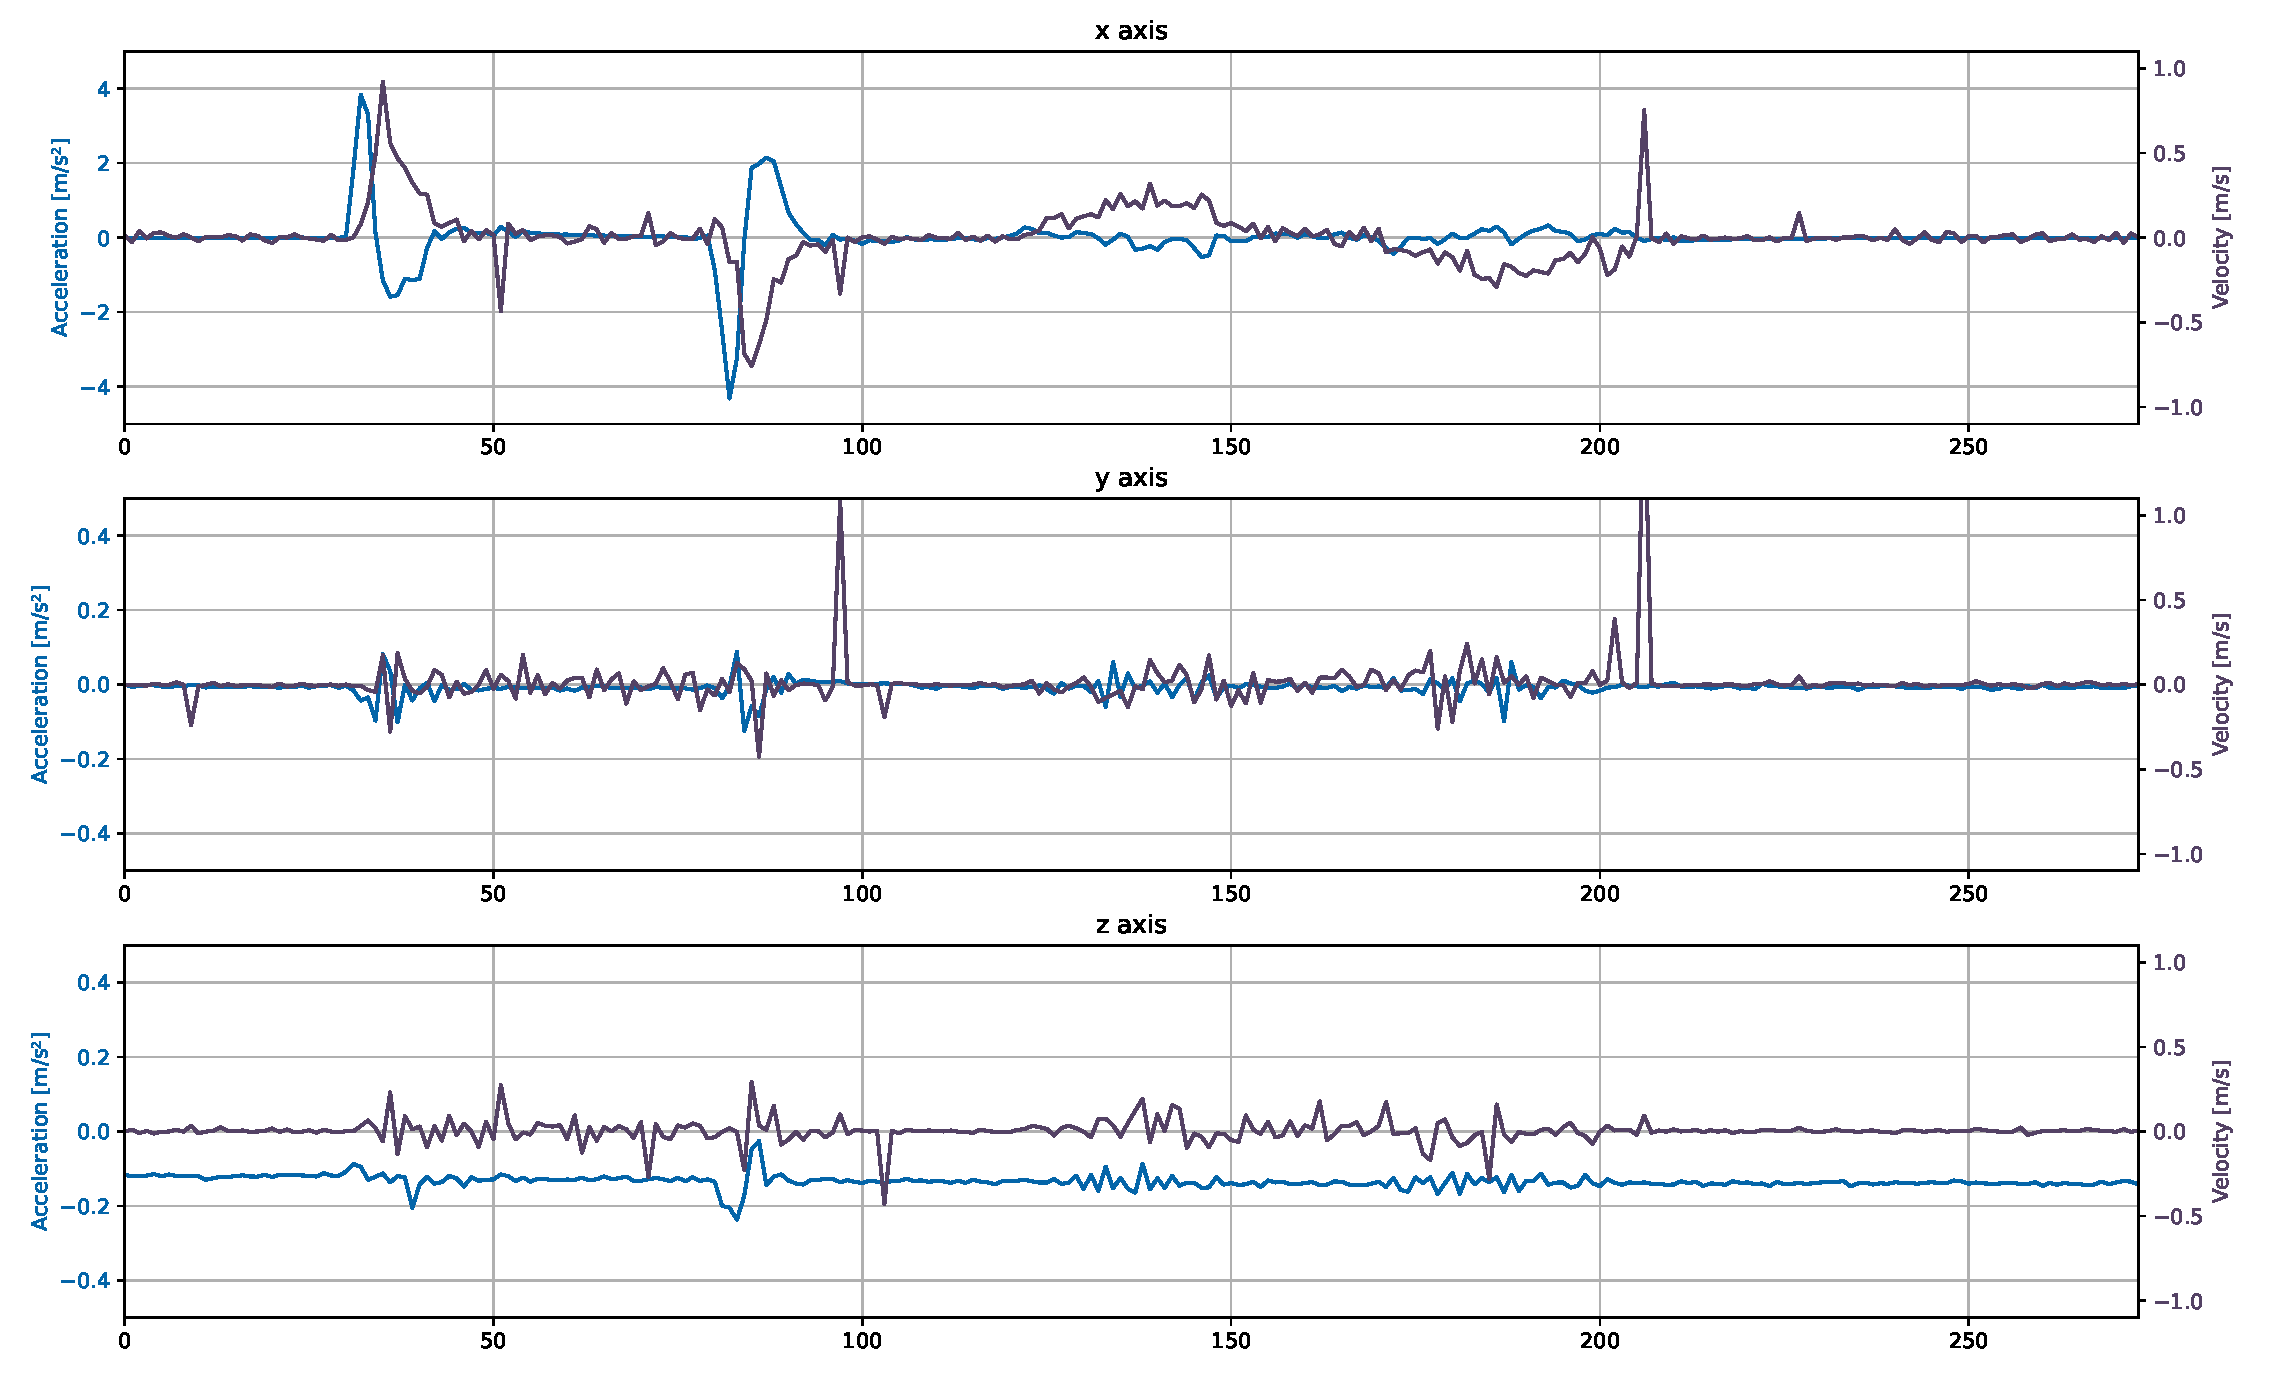
\includegraphics[width=1.0\textwidth]{images/tof_translation_measurement_x.eps}
  \caption{Raw measurement of the translation alongside the x-axis. Before and around 50, the camera is slid fast forward, kept in pause just to slide back before reaching frame number 100. After 100 and before 220, the same motion is repeated but slower. Blue is the acceleration and purple the velocity.}
  \label{im:tof_translation_measurement_x}
\end{figure}
\begin{figure}[H]
  \centering
  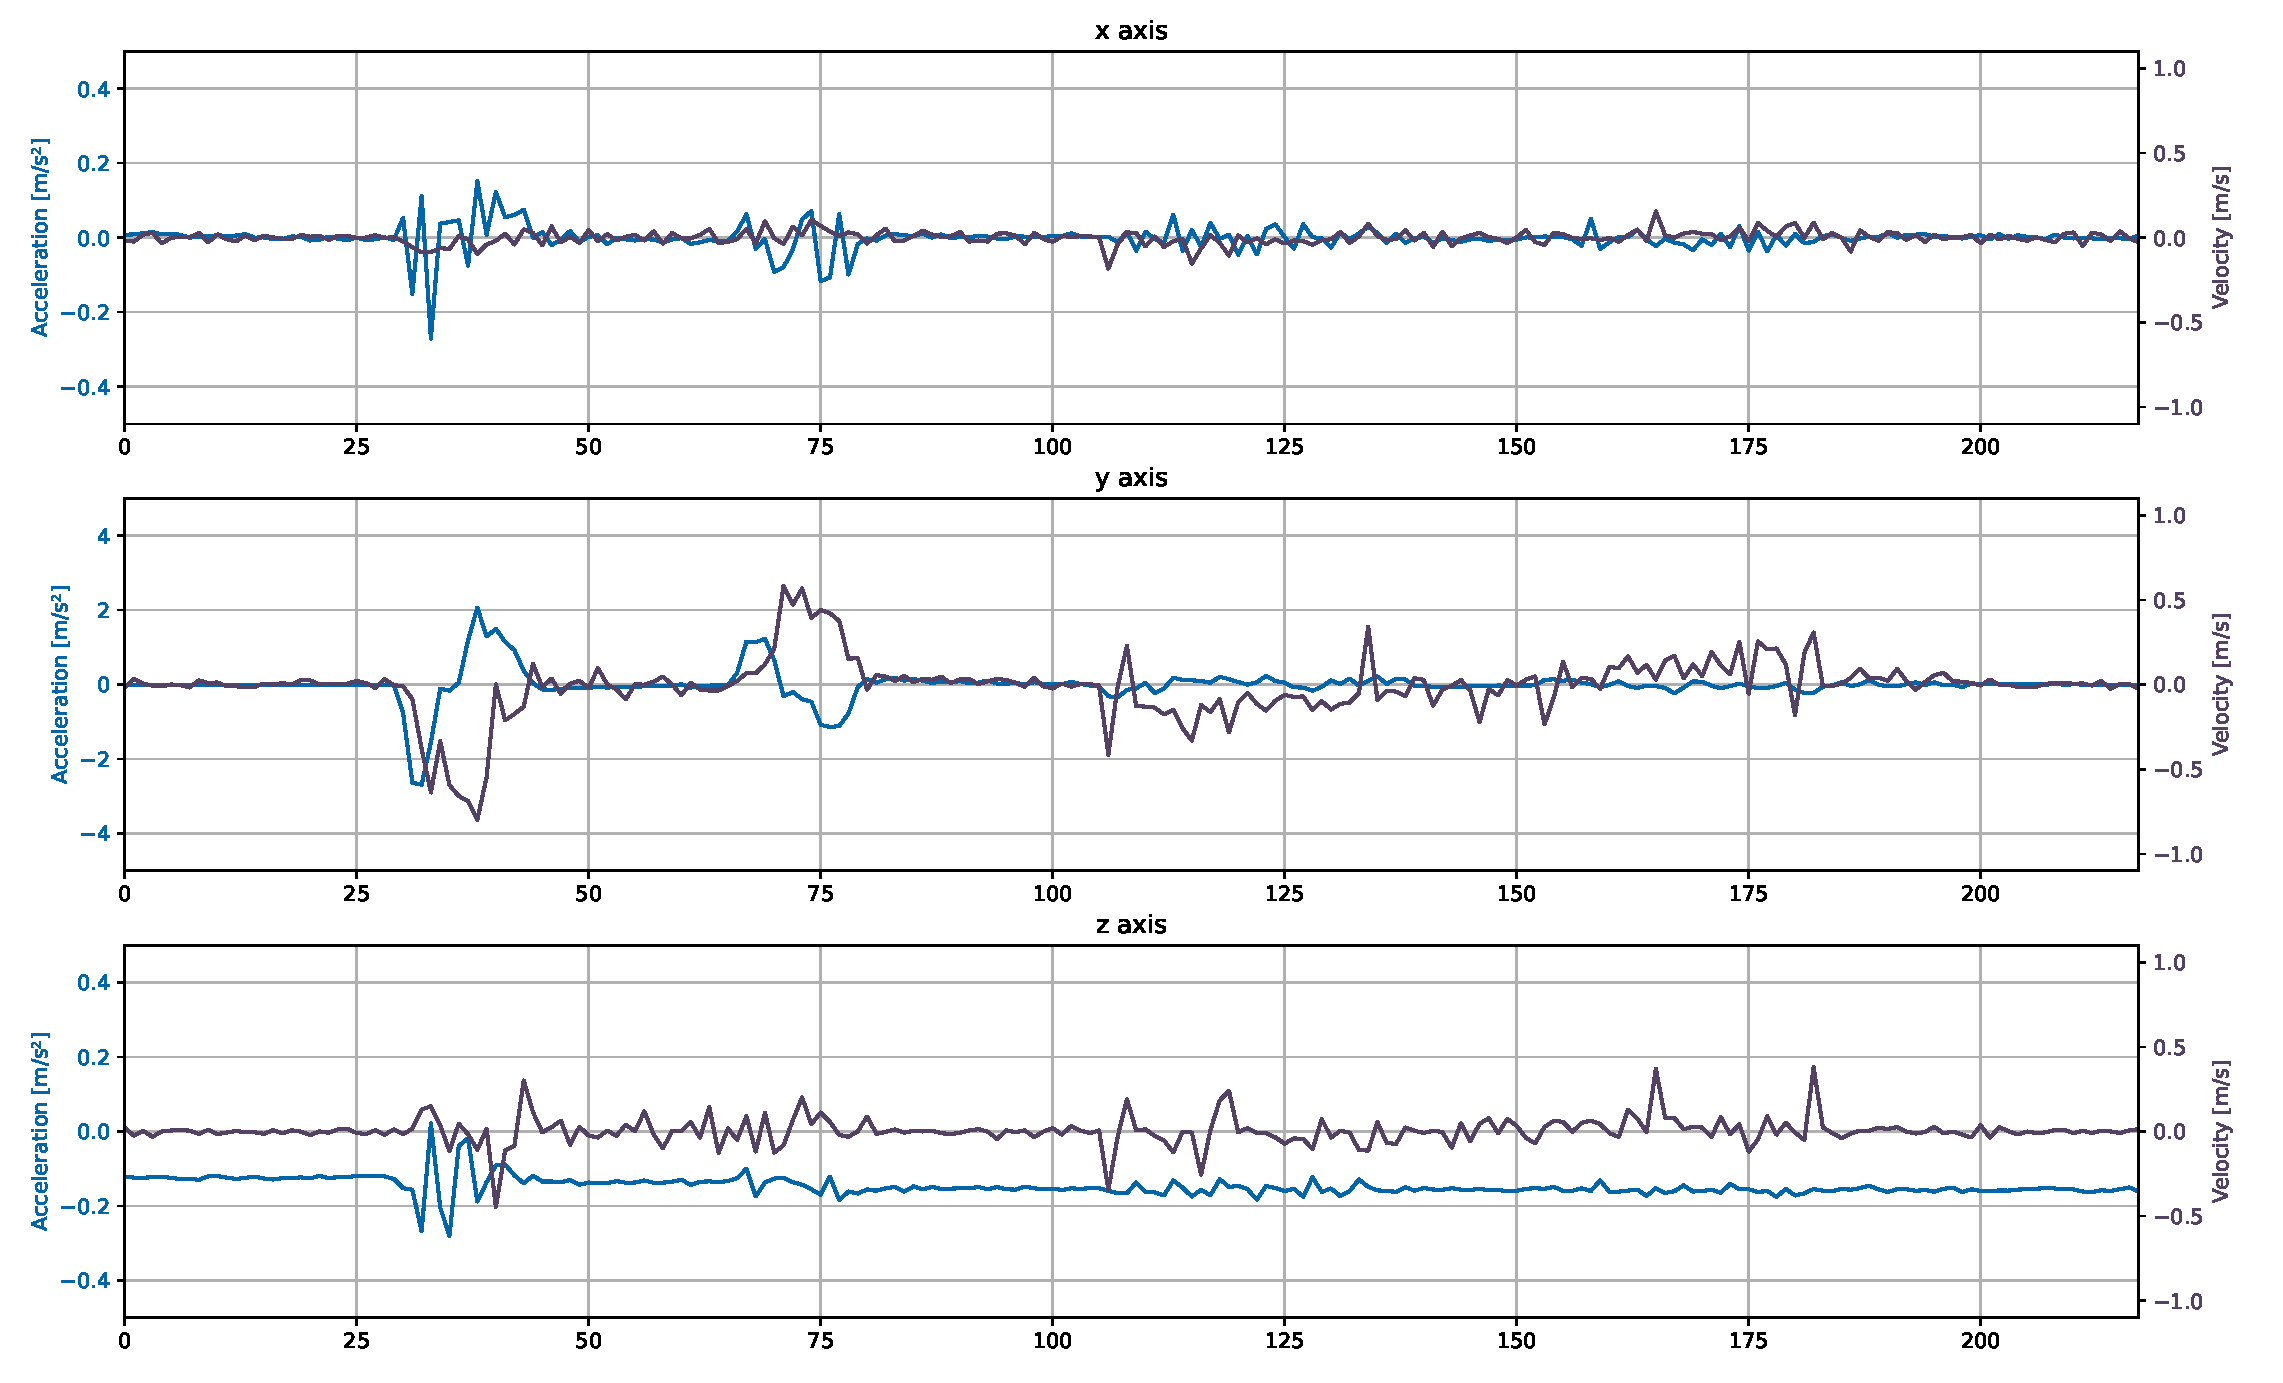
\includegraphics[width=1.0\textwidth]{images/tof_translation_measurement_y.eps}
  \caption{Raw measurement of the translation alongside the y-axis. Between the frames 25 and 50, the camera is slid to the right, kept there and slid back to the origin around frame 75. The motion is repeated slower after frame 100 and before 200. Blue is the acceleration and purple the velocity.}
  \label{im:tof_translation_measurement_y}
\end{figure}
Raw integration of the ToF velocity values gives insight into the measurement's quality. As visible in image \ref{im:tof_translation_measurement_integrated}, the data reconstructs the linear motion in both directions, even though it gets jagged by noise as expected from theory. Noteable outliers, like at the end of the second motion on the x-axis, induce larger errors. 
\begin{figure}[H]
  \centering
  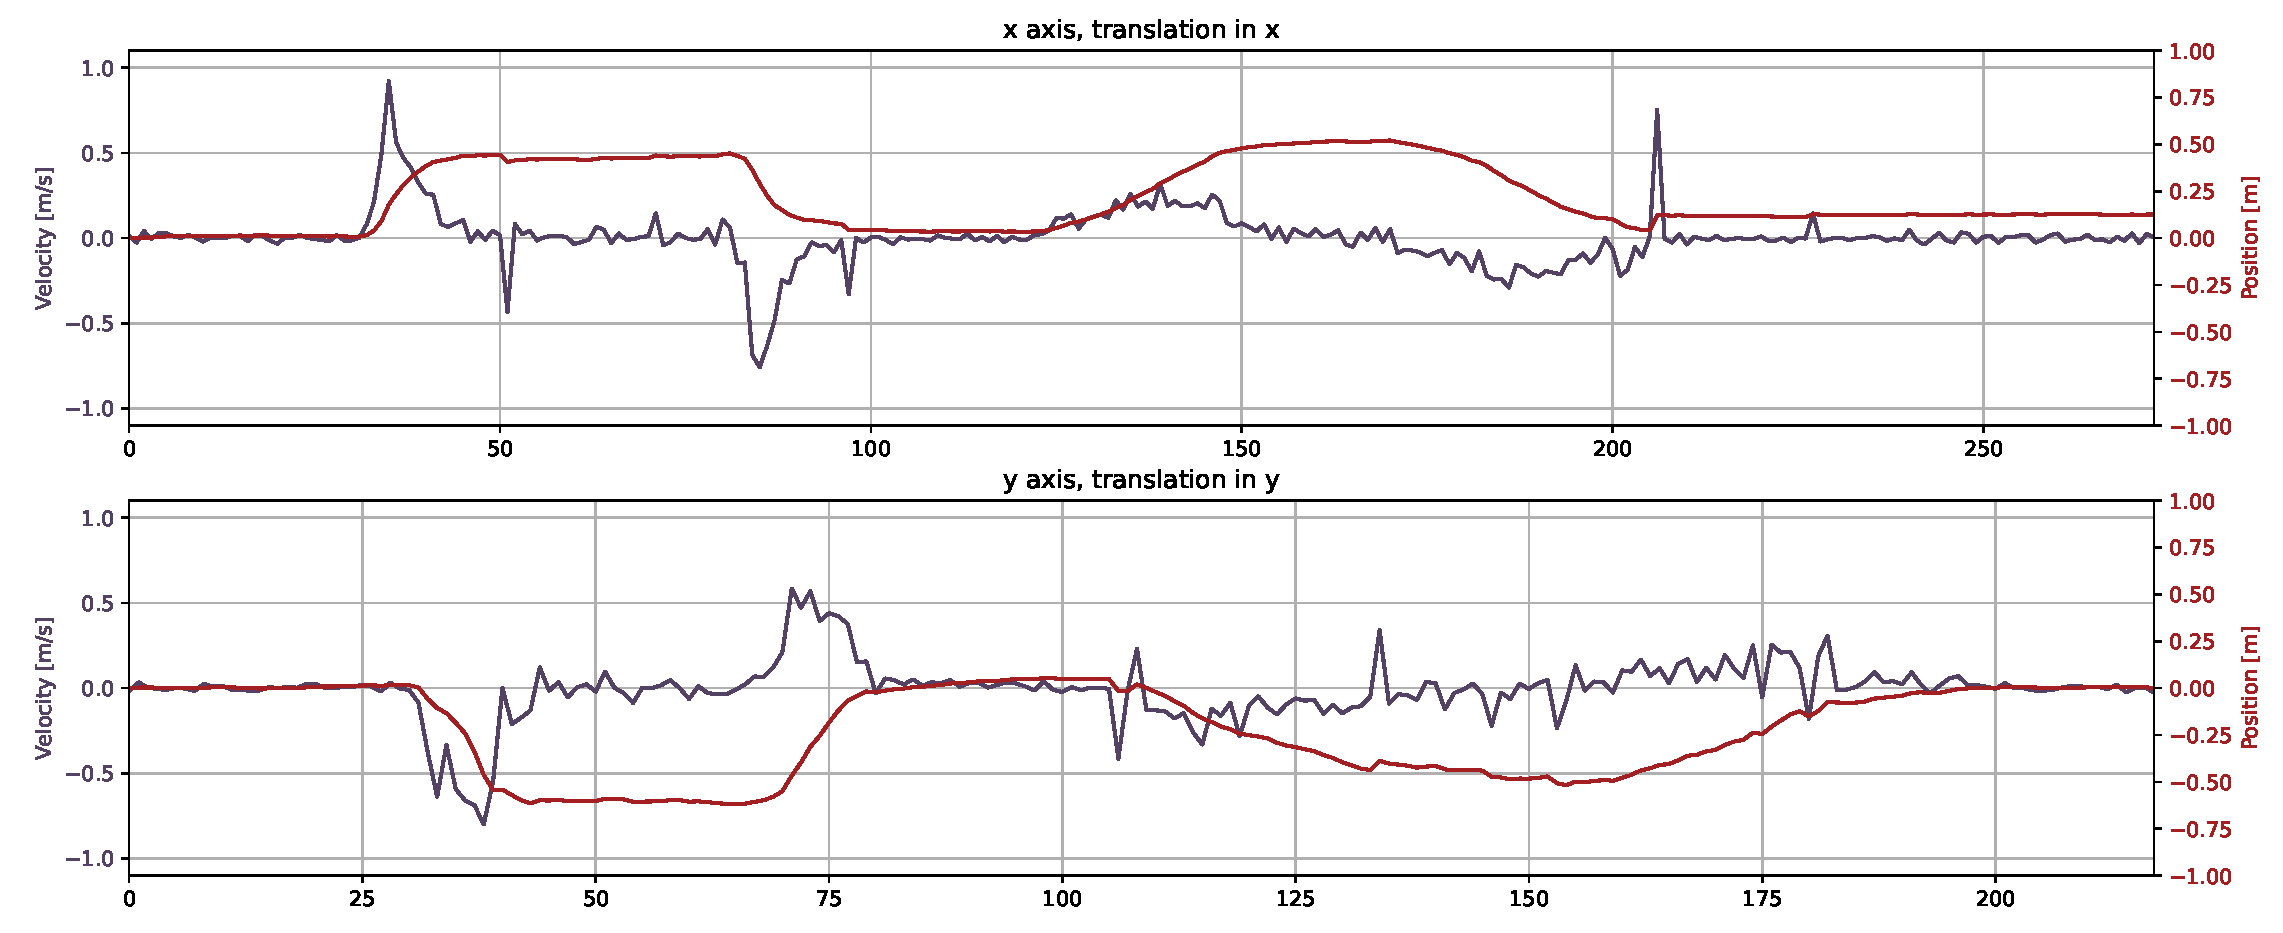
\includegraphics[width=1.0\textwidth]{images/tof_translation_measurement_integrated.eps}
  \caption{Raw integration of the relevant axis in both translations of the ToF velocity data. Red: ToF velocity, Blue: Its integration.}
  \label{im:tof_translation_measurement_integrated}
\end{figure} 
\section{Inertial Measurement Unit}
\label{sec:IMU_results}
The Inertial Motion Unit (IMU) contains a gyroscope and an accelerometer, whose data inputs the Kalman filter. While the comparison to the rotation estimation from the ToF camera already covered the gyroscope in section \ref{sec:results_tof_rotation}, the accelerometer data requires more profound analysis.
\subsection{Accelerometer}
\label{sec:accel_results}
An accelerometer within the gravitational field of the earth will always measure the earth's gravitational pull in addition to other accelerations. The accelerometer needs calibration on each axis to compensate for the gravitational force, so the subtraction of $\vec{g}$ works in any orientation. Experimentation with the accelerometer has shown that a hysteresis prevents the accelerometer from reaching zero or $\vec{g}$ when standing still, depending on prior rotation. The hysteresis leads to a tiny offset on the acceleration, which bleeds into an integrated velocity and devastatingly affects the further integrated position, as visible in image \ref{im:accelometer_integrated} on the next page. The offset is easily visible in images \ref{im:tof_translation_measurement_x} and \ref{im:tof_translation_measurement_y} on the z-axis, thanks to the narrowed scale.\\
The added offset error worsens the drift compared to the simulation in section \ref{sec:Kalmanfilter} dramatically. The integration to the velocity draws a smoother curve, than compared to the raw data of the ToF camera, but a drift is present. The third plot - of the z-axis - shows the devastating drift, if the gravitational pull is not compensated entirely. The data for the third plot got recorded during the measurement of the motion alongside the x-axis.
\begin{figure}[H]
  \centering
  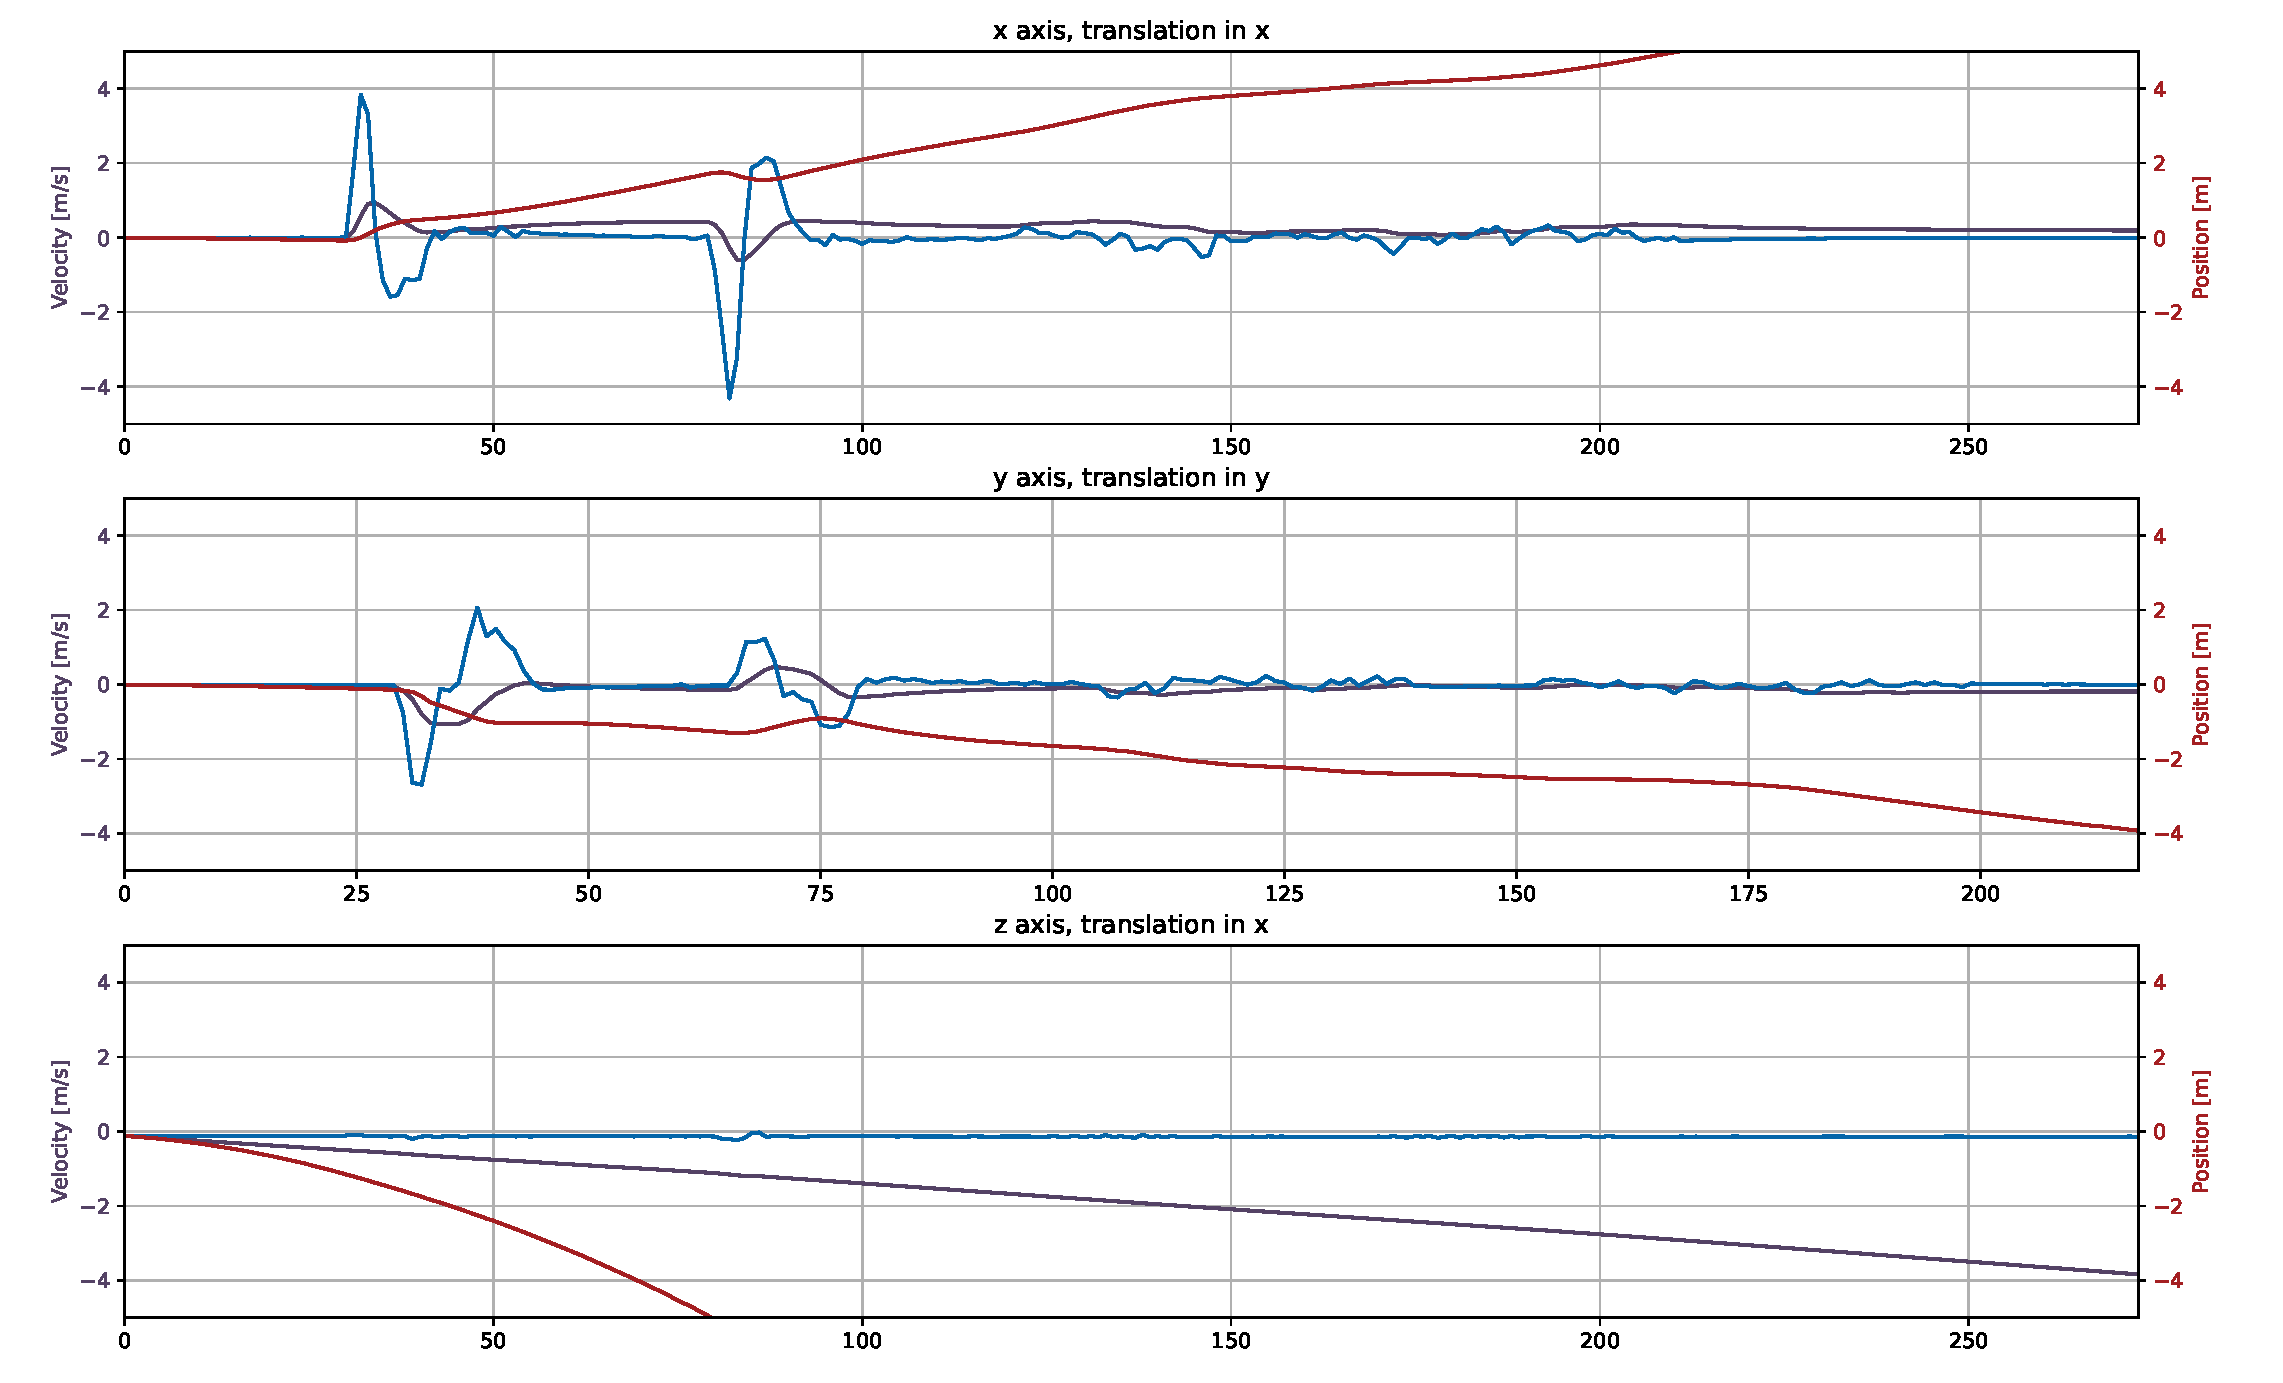
\includegraphics[width=1.0\textwidth]{images/accelerometer_translation_drift.eps}
  \caption{Raw integration of the relevant axis in both translations of the accelerometer. Blue is the acceleration, purple the velocity (single integration) and red the position (double integration).}
  \label{im:accelometer_integrated}
\end{figure} 
\section{Kalman Filter}
\label{sec:kalman_results}
The Kalman filter combines the known motion model of the camera head with the measurement uncertainties and the raw input data from the ToF camera and the IMU. Both types of motion – rotation and translation – are calculated in one large matrix but mostly decoupled. The only coupling between the rotation and the translation is the transformation from ABC-coordinates to the XYZ-space. The rotation is required for the translation data; it gets analyzed first.
\subsection{Rotation}
\label{sec:kalman_rotation_results}
As mentioned in section \ref{sec:results_tof_rotation}, the gyroscope and the ToF camera generate a rotation speed of comparable magnitude and shape. The gyroscope data is less distorted by noise, which gives this sensor more weight in the Kalman filter. 
The Kalman filter smoothes data for the rotation speed through its model function and calculates the rotation through an integration step. Additional to the gyroscope and the ToF camera, the drift compensation with the accelerometer stabilizes the values when the camera head is stationary.\\ 
As explained in section \ref{sec:SensorFusion}, the integration step is a quaternion multiplication of the prior value with the new rotation speed.\\
When plotting the output of the Kalman filter against the raw data of the gyroscope and the ToF camera, the strong weight towards the gyroscope becomes apparent, as shown in figure \ref{im:meas_kalman_rotation} on the next page.\\
Without a reference measurement, it isn't easy to classify these results. The demonstration in figure \ref{fig:rotation_demo} of the whole pipeline using only rotation data helps estimate the result's quality. The three rotation axes of the camera tripod do not intersect with the recording Raspberry Pi camera; therefore, the 3D object is expected to move within the camera image. While the gyroscope's rotation axes intersect in the housing of the IMU, the axes of the ToF camera intersect at the optical center of the lens. For better accuracy, these sensor- and camera displacements on the camera head require additional compensation. 
\begin{figure}[H]
  \centering
  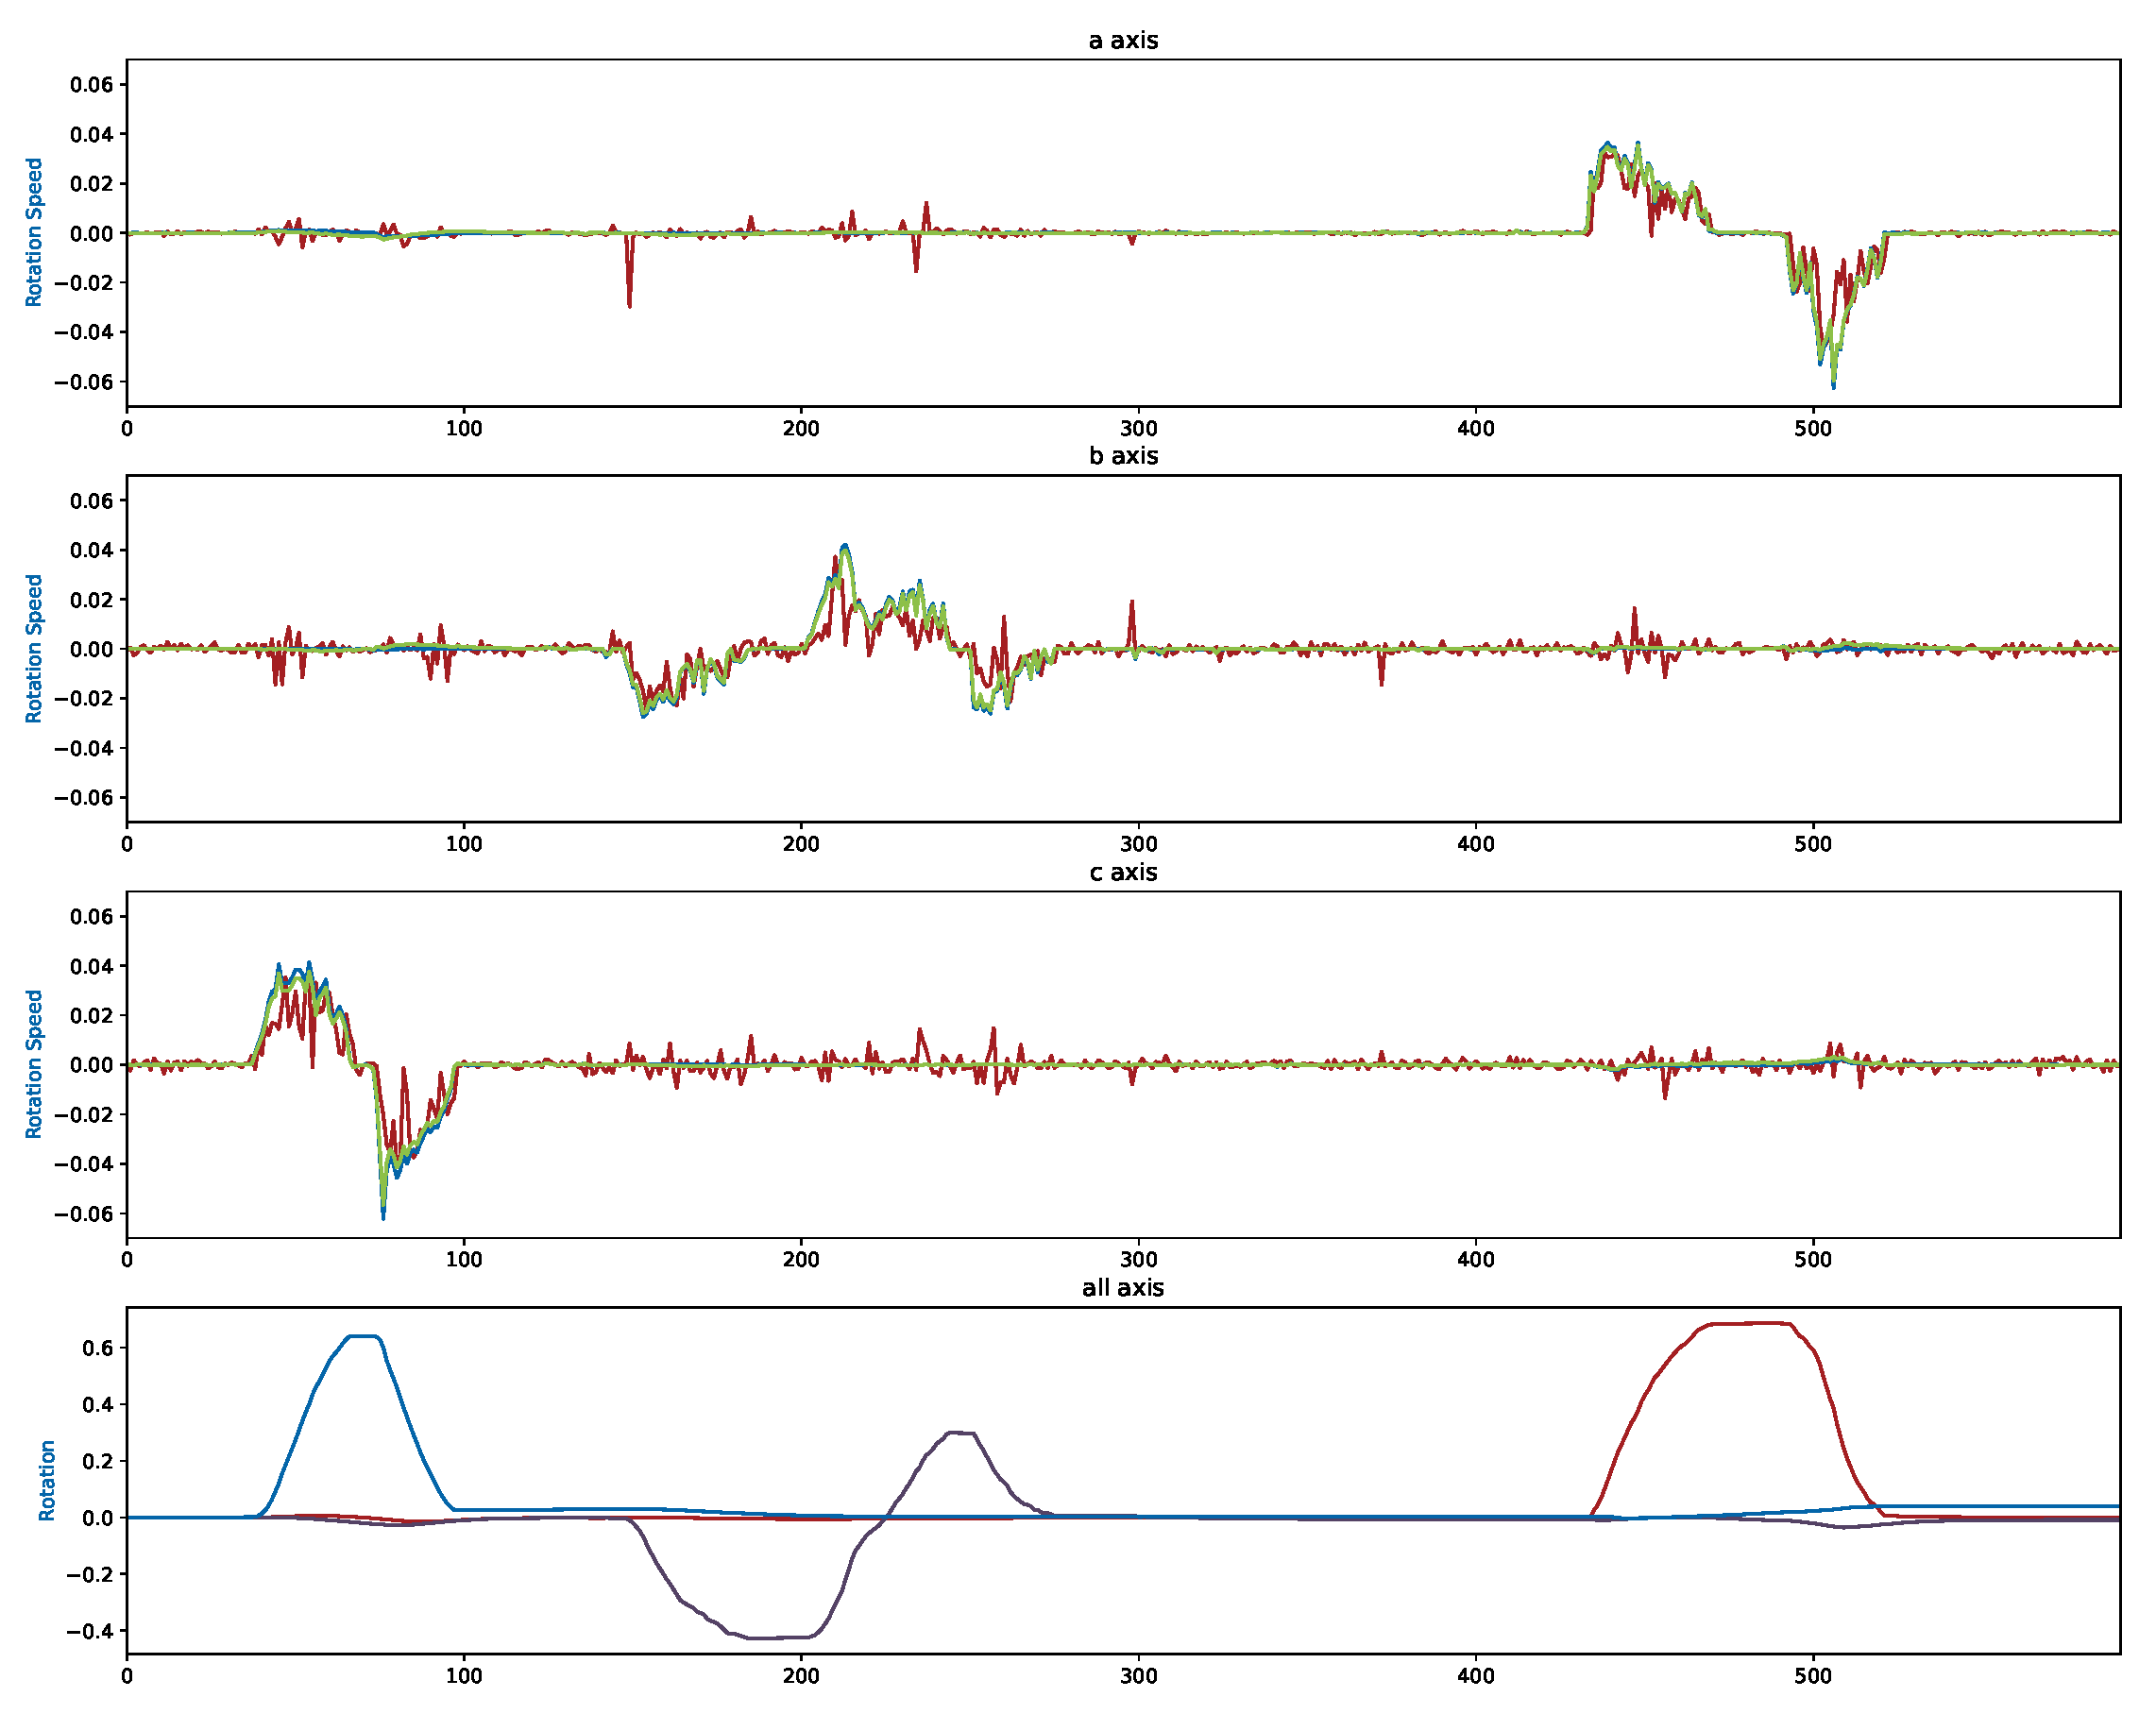
\includegraphics[width=1.0\textwidth]{images/meas_kalman_rotation.eps}
  \caption{The output of the Kalman filter is plotted in green, against the gyroscope data in blue and the ToF camera data in red in the upper three graphs. The fourth graph shows the calculated rotation. The a-axis in red, the b-axis in purple and the c-axis in blue.}
  \label{im:meas_kalman_rotation}
\end{figure} 
\begin{figure}[H]
  \centering
  \begin{minipage}[b]{0.47\textwidth}
    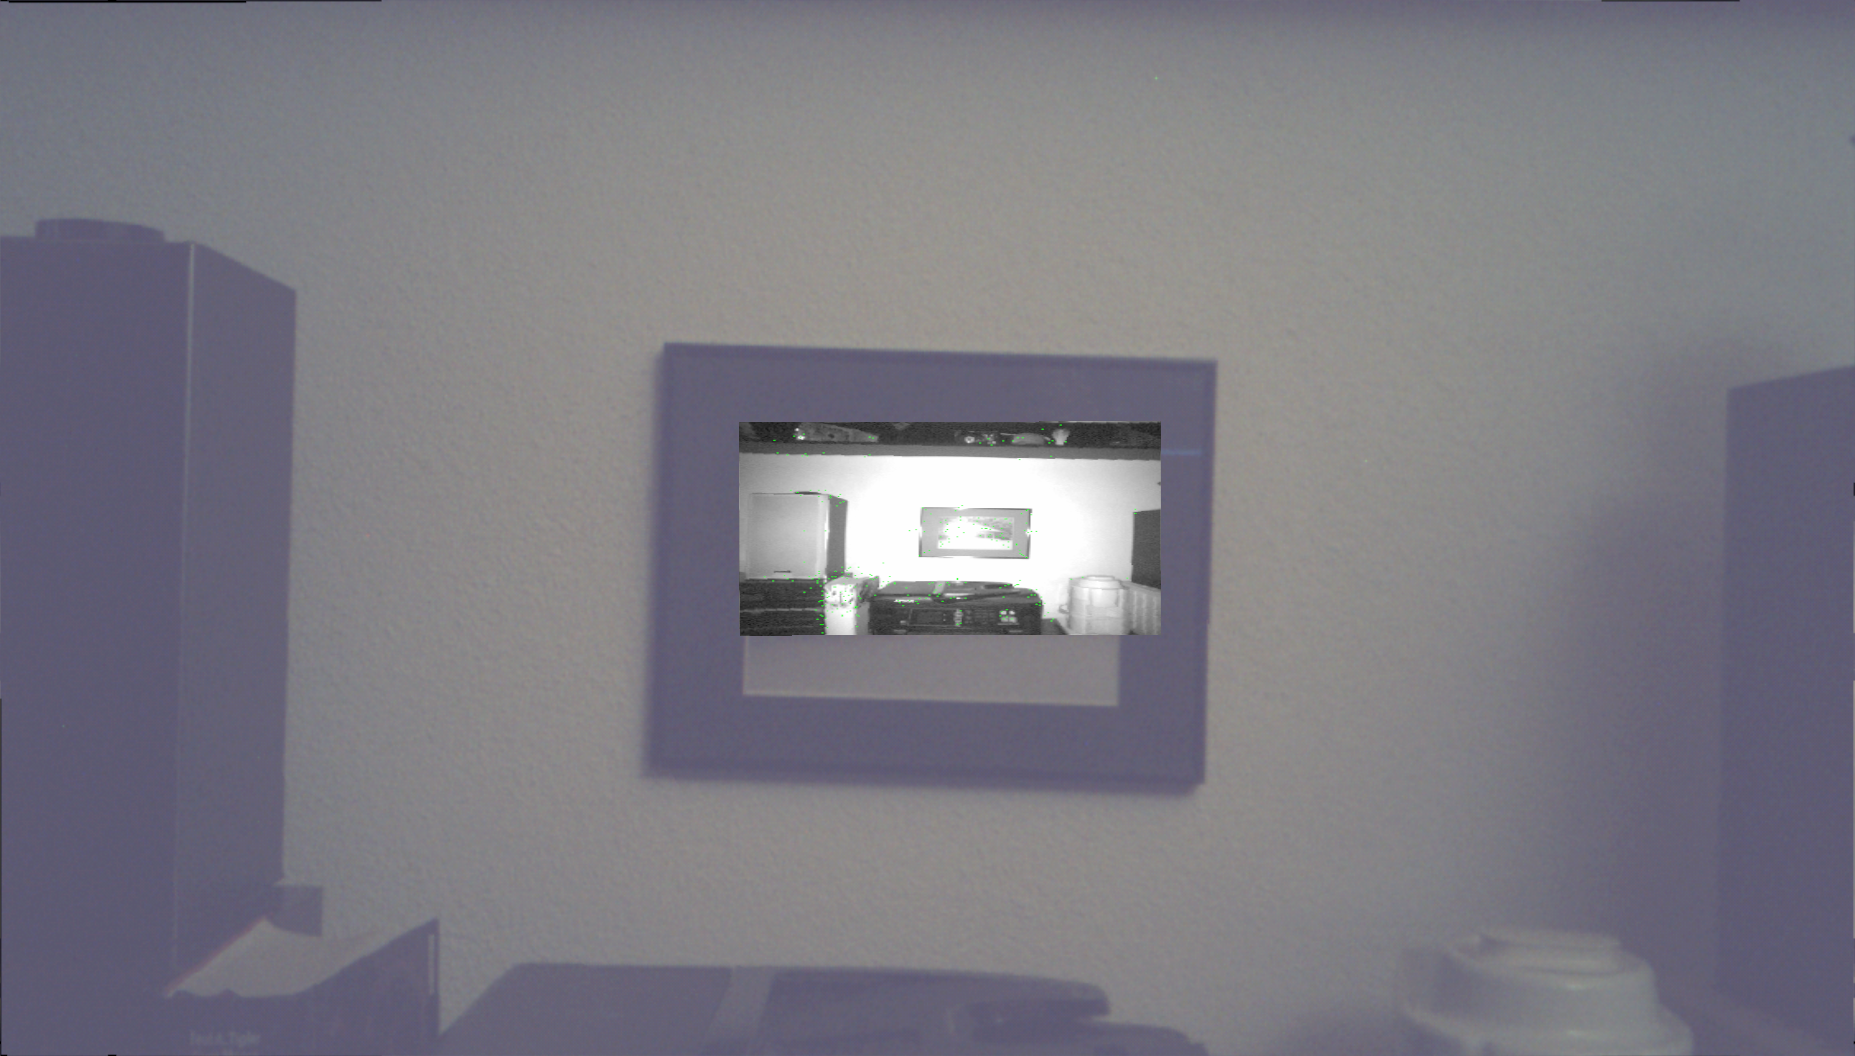
\includegraphics[scale=0.1115]{images/demo_rotation_init.png}
    \caption{Initial situation}
    \label{fig:rotation_demo_init} 
  \end{minipage} % Hier darf keine Leerzeile zwischen den beiden Minipages liegen!
  \begin{minipage}[b]{0.47\textwidth}
    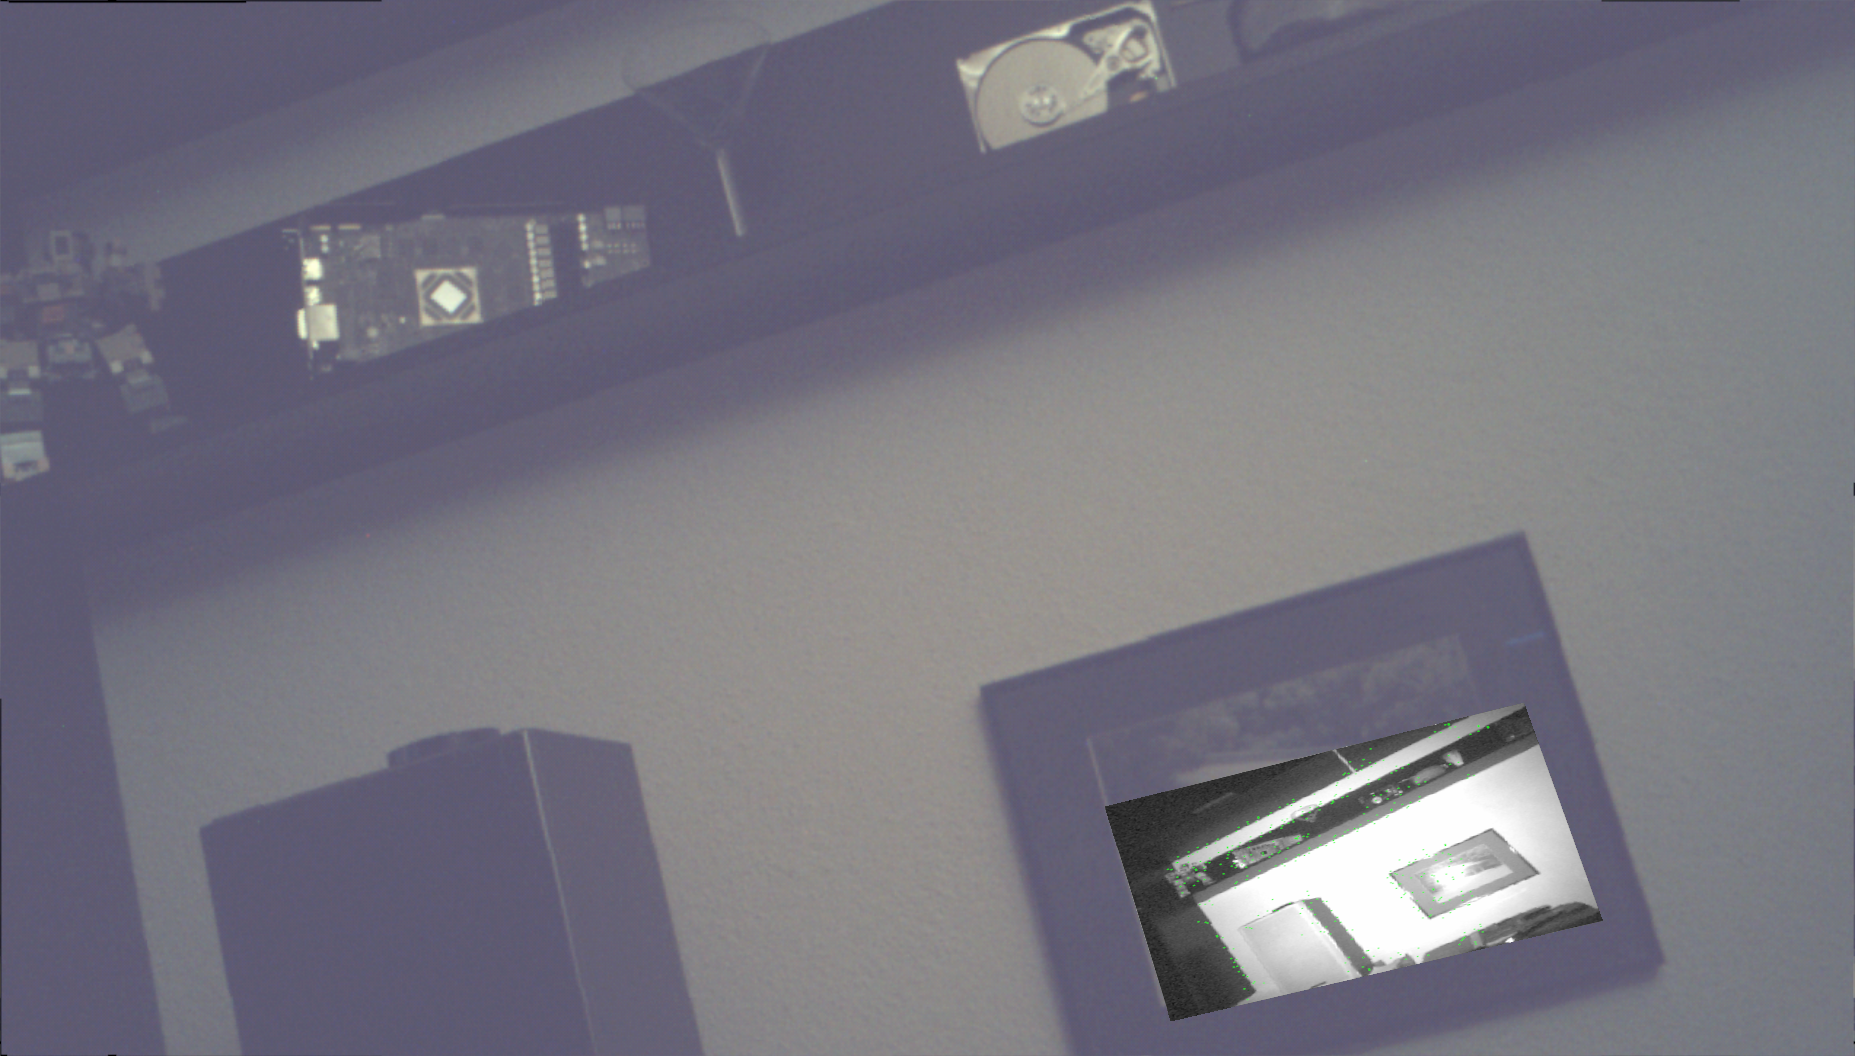
\includegraphics[scale=0.1115]{images/demo_rotation_rotated.png} 
    \caption{After rotation}
    \label{fig:rotation_demo_rotated} 
  \end{minipage}
  \caption{Demonstration of the rotation against the camera image with the moving projection. The displacement of the rectangle inside the picture frame is a result of the Raspberry Pi camera facing translational motion when rotated on the camera tripod.}
  \label{fig:rotation_demo}
\end{figure}
\subsection{Translation}
\label{sec:kalman_translation_results}
The fusion of the accelerometer data and the velocity data from the ToF camera has been simulated in section 222. The simulation did not consider that an offset taints the accelerometer data, leading to an even faster drift on its integrations. Figure 333 shows the output of the Kalman filter in green against the data from the accelerometer in blue and the ToF camera in red. Lacking any other input to compare against, the Kalman filter follows the accelerometer directly; the blue line is hidden behind the green Kalman output. The accelerometer's integration curve compares directly against the raw ToF camera data and the Kalman filter output on the velocity. Further integration allows the comparison with the positional data.\\
Arguably, the accelerometer taints the Kalman filter data, rendering it worse than the raw integration of the ToF camera. The Kalman velocity output is significantly worse than in the simulation, the proposed integration on this output, to get even better positional data fails.
\begin{figure}[H]
  \centering
  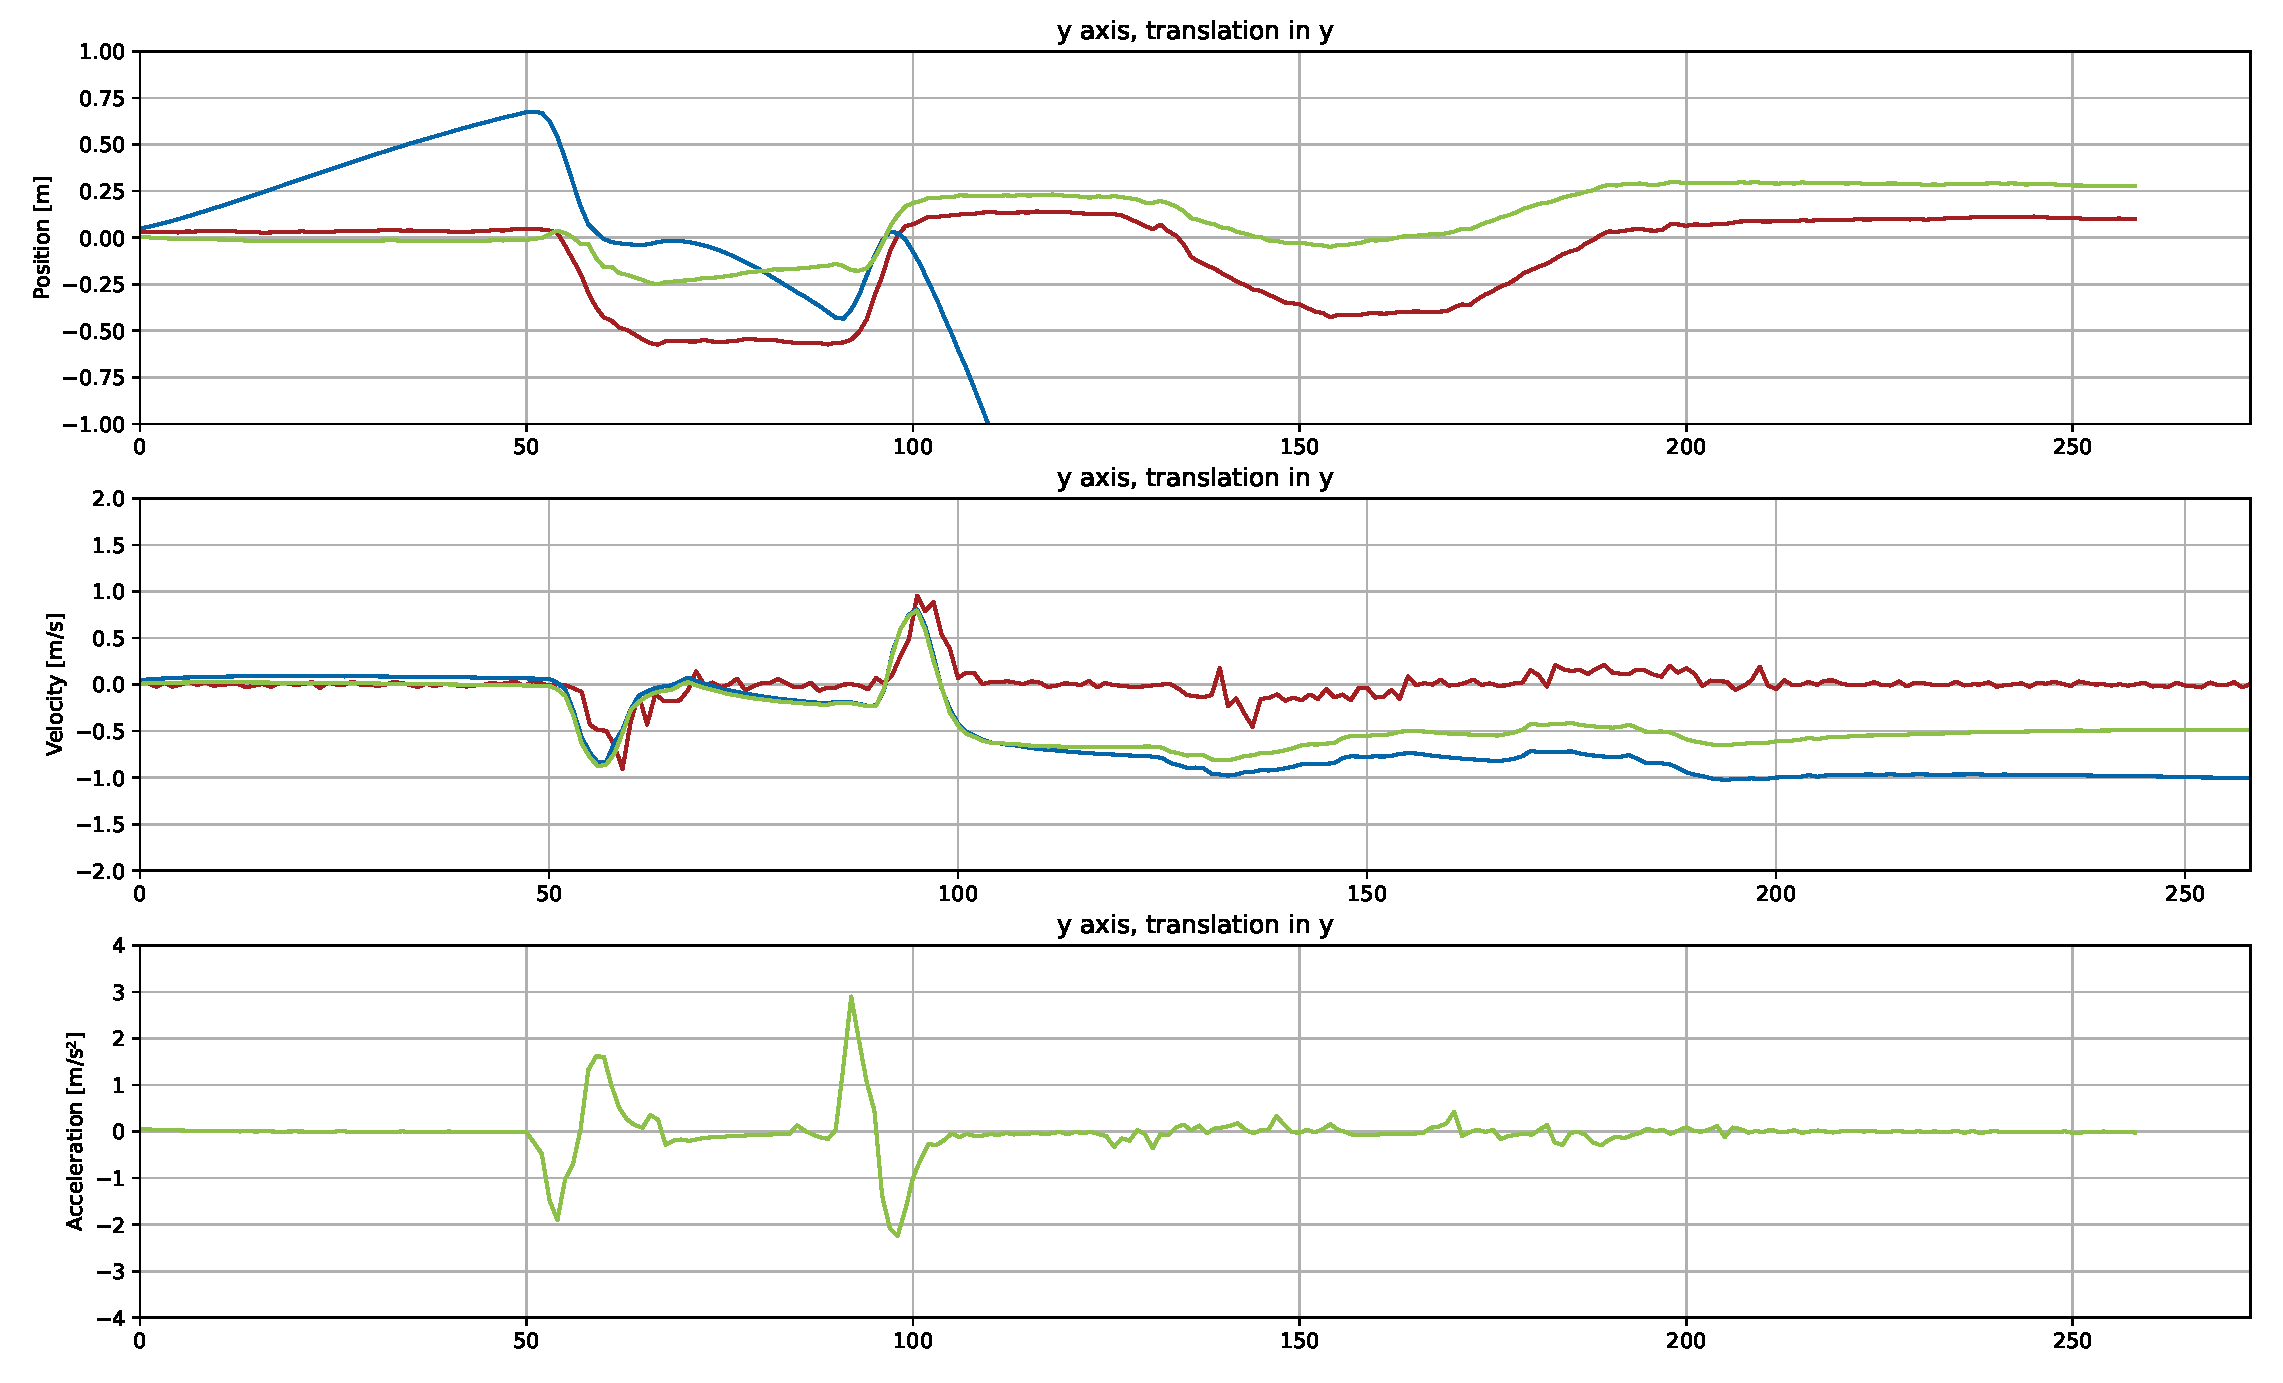
\includegraphics[width=1.0\textwidth]{images/measurement_kalman_translation.eps}
  \caption{Motion in y direction. Blue lines are data from the accelerometer and its integrations, red are the velocity from the ToF camera and its integration and in green are the different Kalman outputs.}
  \label{im:meas_kalman_translation}
\end{figure} 